\documentclass[10pt,xcolor=table]{beamer}

\usetheme[subsectionpage=progressbar]{metropolis}

\usepackage{FiraSans}
\setsansfont[BoldFont={FiraSans-Regular},ItalicFont={FiraSans-LightItalic},BoldItalicFont={FiraSans-Italic}]{FiraSans-Light.otf}
\usepackage{FiraMono}
\setmonofont[BoldFont={FiraMono-Medium}]{FiraMono-Regular.otf}

\setbeamertemplate{itemize subitem}{--}
\setbeamerfont{caption}{size=\footnotesize}
\usepackage{appendixnumberbeamer}

\usepackage{listings}
\lstset{
  basicstyle=\footnotesize\ttfamily,
  backgroundcolor = \color{gray!20}
}
\lstdefinestyle{c}{language=C,
  keywordstyle=\bfseries\color{green!40!black},
  commentstyle=\itshape\color{purple!40!black},
  % identifierstyle=\color{blue},
  stringstyle=\color{orange}
}
\lstdefinestyle{shell}{language=sh,
  commentstyle=\itshape\color{purple!40!black},
  moredelim=**[is][\only<2->{\color{red}}]{@}{@},
  moredelim=**[is][\only<3>{\color{blue}}]{¿}{¿}
}
\lstdefinestyle{asm}{language=[x86masm]Assembler,
  commentstyle=\itshape\color{purple!40!black},
}
\lstdefinestyle{valgrind}{basicstyle=\footnotesize\ttfamily,
  backgroundcolor = {},
}
\usepackage{caption}
\captionsetup[lstlisting]{font={small,tt}, labelformat=empty,
  labelsep=none}

\usepackage{booktabs}
\usepackage[scale=2]{ccicons}

\usepackage{pgfplots}
\usepgfplotslibrary{dateplot}

\usepackage{expl3}
\ExplSyntaxOn
\int_zero_new:N \g__prg_map_int
\ExplSyntaxOff
\usepackage{tikz}
\usetikzlibrary{tikzmark,decorations.pathreplacing,calligraphy}

% Figure's path
\graphicspath{{./figs/}}


\title{Optimization and Profiling of HPC Applications}
\subtitle{using free software resources}
\date{\today}
\author{Emilio J. Padrón González}
 \institute{\href{mailto:emilioj@udc.gal}{\nolinkurl{emilioj@udc.gal}}
   -- \url{http://gac.udc.es/~emilioj}\\Computer Architecture Group
   -- Universidade da Coruña}

\begin{document}

\maketitle

\begin{frame}{Outline}

  \setbeamertemplate{section in toc}[sections numbered]
  \tableofcontents[hideallsubsections]

\end{frame}

\begin{frame}{Contents: Lessons 1 and 2}

  \setbeamertemplate{section in toc}[sections numbered]
  \setbeamertemplate{subsection in toc}[ball unnumbered]
  \tableofcontents[sections={1-2}]

\end{frame}

\begin{frame}{Contents: Lessons 3 and 4}
  \setbeamertemplate{section in toc}[sections numbered]
  \setbeamertemplate{subsection in toc}[ball unnumbered]
  \tableofcontents[sections={3-4}]
\end{frame}

\begin{frame}{Contents: Lesson 5}
  \setbeamertemplate{section in toc}[sections numbered]
  \setbeamertemplate{subsection in toc}[ball unnumbered]
  \tableofcontents[sections={5}]
\end{frame}


\section{Introduction}

\subsection{Free Software}

\frame{
  \frametitle{What we means by: [\ldots] using \underline{Free
      Software} resources}

  \begin{tikzpicture}[remember picture,overlay]
    \node[xshift=-2cm,yshift=-2.5cm] at (current page.north east) {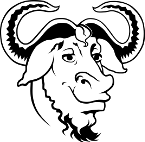
\includegraphics[width=2cm]{gnu.png}};
  \end{tikzpicture}

  \vfill

  \begin{quote}
    Free as in Freedom~\footnote{\ldots not as in \emph{free beer}: \url{http://www.oreilly.com/openbook/freedom}}
  \end{quote}

  \vfill

  \begin{itemize}
  \item Free software definition according to FSF:
    \url{http://www.gnu.org/philosophy/free-sw.html}
  \item Similar terms: \emph{Open Source}, \emph{FLOSS} (Free/Libre
    and Open Source Software)
  \end{itemize}
}

\subsection{Computer architecture basics}

\frame{
  \frametitle{Computer organization: CPU, Mem \& I/O}

  \begin{figure}
    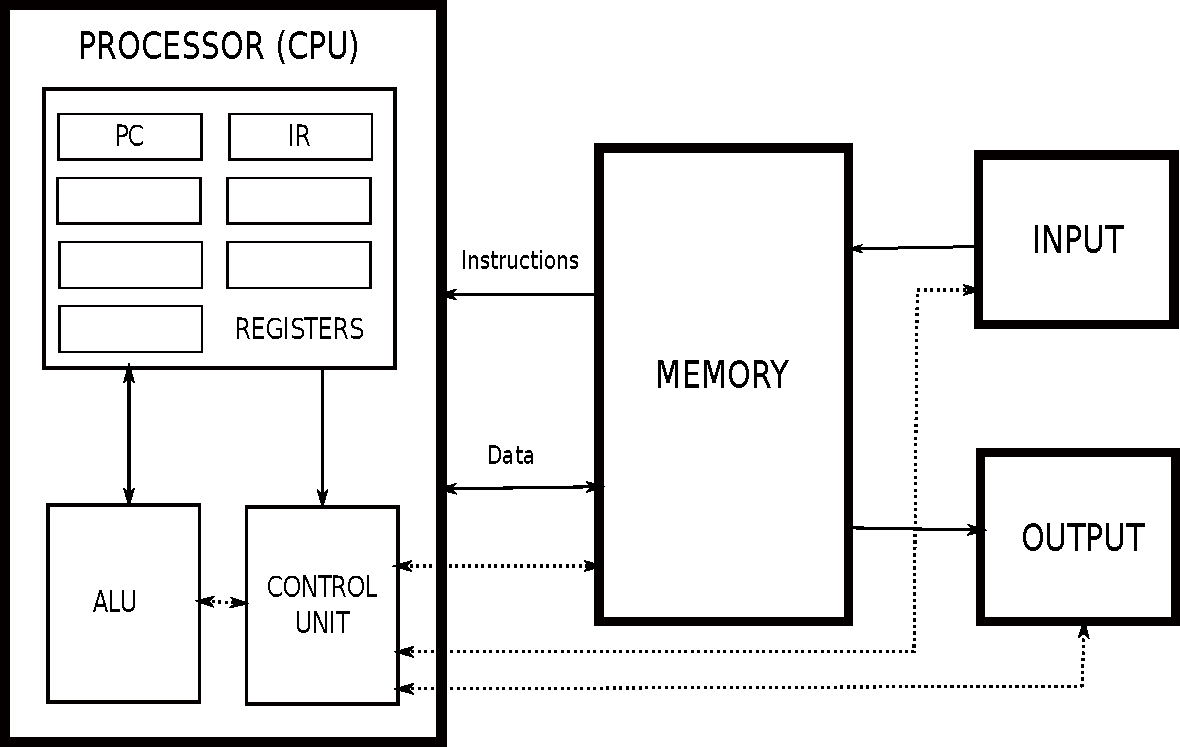
\includegraphics[width=\textwidth]{computerstruct}
    \caption{3 main subsystems of a computer: CPU, Memory and Input/Output}
  \end{figure}
}

\frame{
  \frametitle{The processor}

  \begin{block}{Basically\ldots}
    Carries out the instructions of a computer program by performing
    the basic {\bf arithmetic}, {\bf logical}, {\bf control} and {\bf
      I/O} operations specified by the instructions.
  \end{block}

  \begin{columns}
    \column{0.3\textwidth}{
      \begin{figure}
        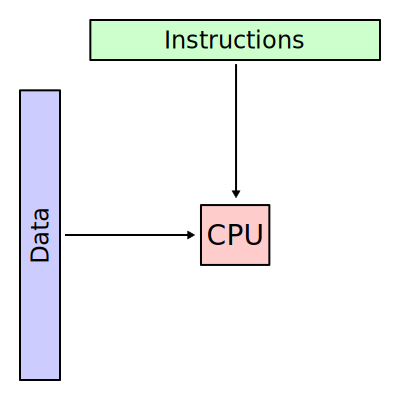
\includegraphics[width=\textwidth]{SISD_alt}
      \end{figure}
    }

    \pause

    \column{0.7\textwidth}{
      \begin{itemize}
      \item[$\Rightarrow$] both Data \& Instructions taken from mem
        \pause
      \item[$\Rightarrow$] common scenario these days: multi-proc/multi-core systems
      \end{itemize}
      \begin{figure}
        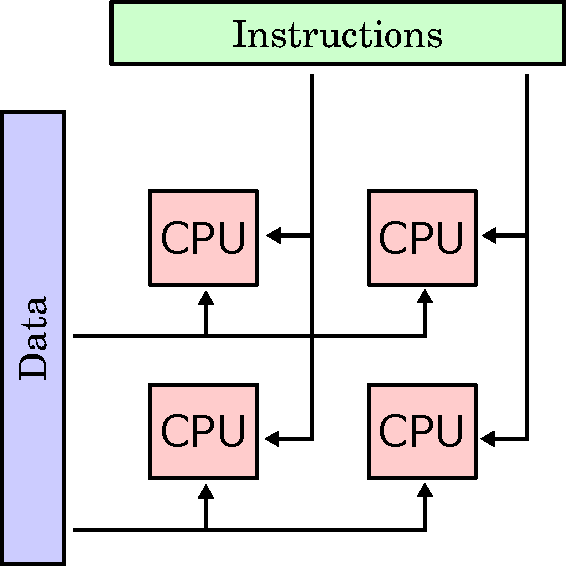
\includegraphics[width=0.4\textwidth]{MIMD_alt}
        \caption*{\ldots more on this later}
      \end{figure}
    }
  \end{columns}
}

\frame{
  \frametitle{The memory}

  \begin{figure}
    \begin{overprint}
      \onslide<1>
      \includegraphics<1>[width=\textwidth]{memhierarchy}
      \onslide<2>
      \includegraphics<2>[width=\textwidth]{memhierarchy_detail}
    \end{overprint}
    \caption{Memory levels in a computer}
  \end{figure}
}

\frame{
  \frametitle{CPU \& Cache memory levels}

  \begin{figure}
    \begin{columns}
      \column{0.4\textwidth}{
        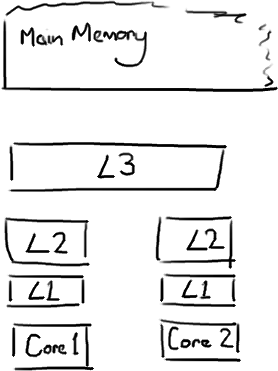
\includegraphics[width=0.5\textheight]{CPUCache}
      }

      \column{0.45\textwidth}{
        \begin{table}\footnotesize
          \caption{Memory latencies from CPU}
          \begin{tabular}{lll}
            \toprule
            \parbox[t]{1.3cm}{\bf Latency\\ CPU to...}
            & \parbox[t]{1.35cm}{\bf CPU cycles\\(approx.)}
            & \parbox[t]{1cm}{\bf Time\\ (approx.)}\\[0.5cm]
            Main mem & & \~{}60-80ns\\
            QPI transit & & \~{}20ns\\
            L3 cache & \~{}40-45 cycles & \~{}15ns\\
            L2 cache & \~{}10 cycles & \~{}3ns\\
            L1 cache & \~{}3-4 cycles & \~{}1ns\\
            Register & 1 cycle\\
            \bottomrule
          \end{tabular}
        \end{table}
      }
    \end{columns}
    \vspace*{-0.4cm}
    \caption{Memory hierarchy in a multi-core CPU~\footnote{2010
        numbers. More up-to-date info:
        \url{http://gist.github.com/eshelman/343a1c46cb3fba142c1afdcdeec17646}}\\
      {\scriptsize By Trisha Gee, CC BY 3.0,
        \url{http://trishagee.github.io/post/dissecting_the_disruptor_why_its_so_fast_part_two__magic_cache_line_padding}}
    }
  \end{figure}
}

\frame{
  \frametitle{Cache and cache lines}

  Cache: exploiting locality
  \begin{itemize}
  \item temporal
  \item spatial
  \end{itemize}

  \pause

  \begin{figure}
    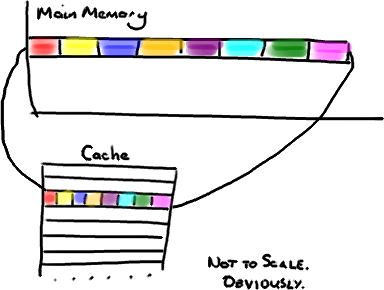
\includegraphics[width=0.75\textheight]{CacheLines}

    \caption{Cache line: transfer unit L1 <-> L2 <-> L3 <-> Main mem\\
      {\scriptsize By Trisha Gee, CC BY 3.0,
        \url{http://trishagee.github.io/post/dissecting_the_disruptor_why_its_so_fast_part_two__magic_cache_line_padding}}}
  \end{figure}
}

\frame{
  \frametitle{Cache behavior is \underline{key} for performance}

  \begin{figure}
    \quad

    \begin{overprint}
      \onslide<1>\centering
      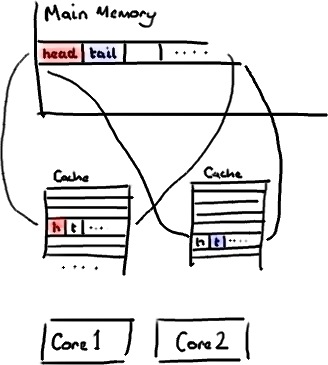
\includegraphics[width=0.65\textheight]{FalseSharing}
      \onslide<2>\centering
      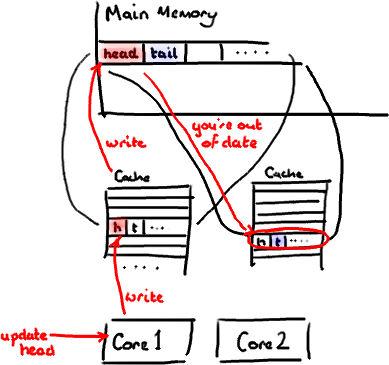
\includegraphics[width=0.7\textheight]{FalseSharingWriteHead}
      \onslide<3>\centering
      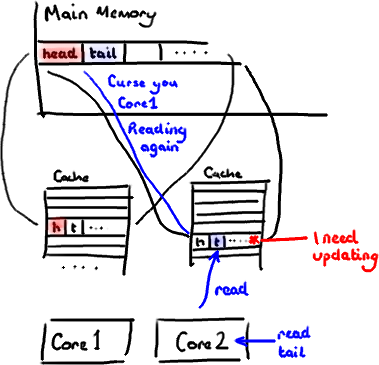
\includegraphics[width=0.7\textheight]{FalseSharingReadTail}
          \end{overprint}
    \caption{Example of cache misbehavior: {\bf False sharing}\\
      {\scriptsize By Trisha Gee, CC BY 3.0,
        \url{http://trishagee.github.io/post/dissecting_the_disruptor_why_its_so_fast_part_two__magic_cache_line_padding}}}
  \end{figure}
}

\subsection{HPC basics}

\frame{
  \frametitle{Forms of parallel computing}

  \begin{itemize}
  \item Bit-level parallelism
  \item Instruction-level parallelism (ILP)
  \item Data-level parallelism (DLP)
  \item Task-level parallelism (TLP)
  \end{itemize}
}

\frame{
  \frametitle{A taxonomy of computer architectures}

  Flynn's taxonomy (1966!)

  \begin{description}
  \item[SISD] Single Instruction stream; Single Data stream
  \item[MISD] Multiple Instruction stream; Single Data stream
  \item[SIMD] Single Instruction stream; Multiple Data stream
    \only<2->{
      \begin{description}
      \item[\alert{\footnotesize (variant)} SIMT] Single Instruction; Multiple Threads
      \end{description}
    }
  \item[MIMD] Multiple Instruction stream; Multiple Data stream
    \only<3>{
      \begin{description}
      \item[\alert{\footnotesize (typically)} SPMD model] Single Program; Multiple Data\\
        \hspace*{-0.4cm} {\small $\Rightarrow$ every task executes the
          same program}
        \vspace*{-0.5cm}
      \end{description}
    }
  \end{description}

  \begin{figure}
    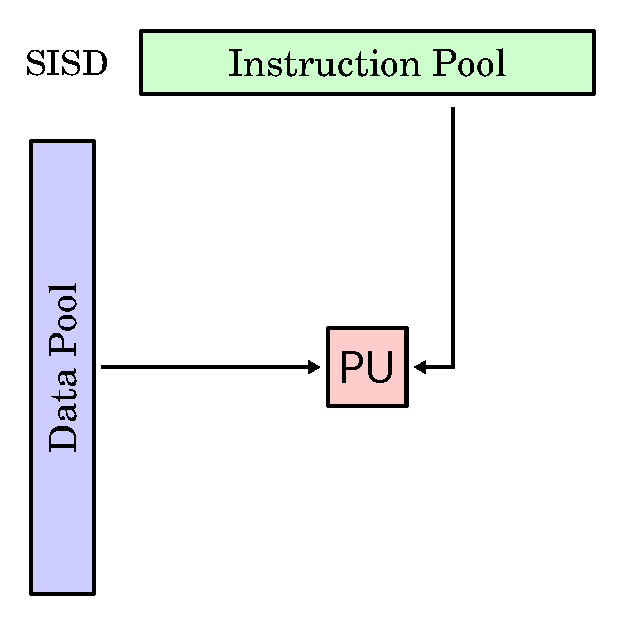
\includegraphics[width=0.25\textwidth]{SISD}~
    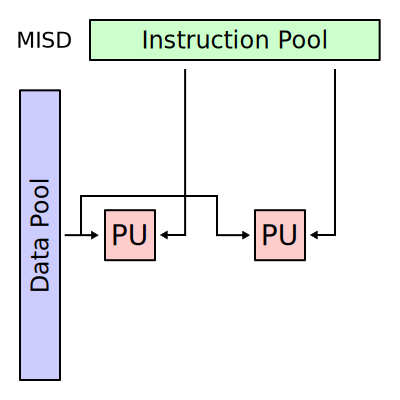
\includegraphics[width=0.25\textwidth]{MISD}~
    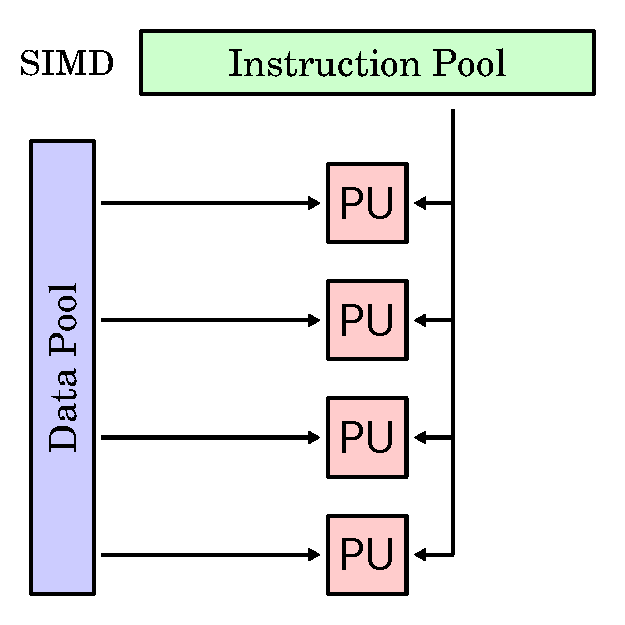
\includegraphics[width=0.25\textwidth]{SIMD}~
    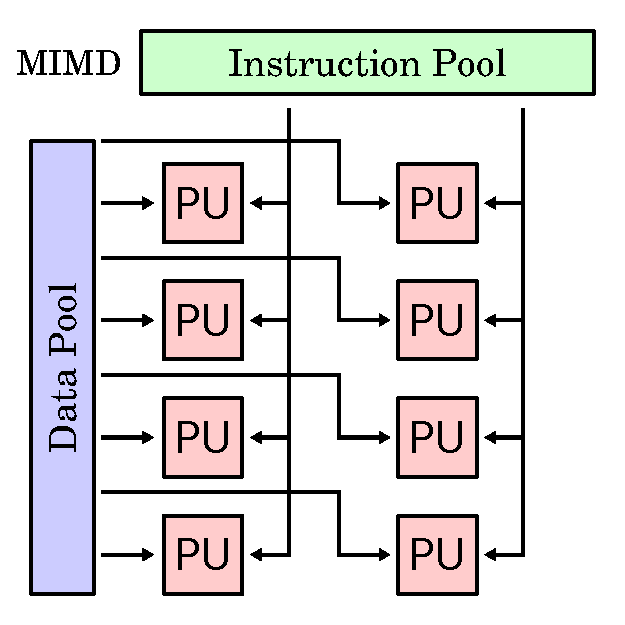
\includegraphics[width=0.25\textwidth]{MIMD}
    \caption{By I, Cburnett, CC BY-SA 3.0,
      \url{https://commons.wikimedia.org/w/index.php?curid=2233537}}
  \end{figure}
}

\frame{
  \frametitle{Parallel processing in Flynn's taxonomy}

  \begin{block}{SISD: exploit ILP}
    \begin{itemize}
    \item Superscalar processors
    \item Pipelining
    \end{itemize}
  \end{block}

  \begin{block}{SIMD: exploit data parallelism}
    \begin{itemize}
    \item Array and Vector processors
    \item Vector extensions in general purpose CPU
    \item GPGPU or similar approaches based on co-processors
    \end{itemize}
  \end{block}

  \begin{block}{MIMD: exploit task parallelism}
    \begin{itemize}
    \item Multicore, multiprocessor and multicomputer architectures
    \end{itemize}
  \end{block}

}

\frame{
  \frametitle{Supercomputers \& HPC Systems}

  \begin{description}
  \item[Monoprocessor with SIMD capabilities] ~
    \begin{itemize}
    \item Exploting the parallelism exposed:
      \begin{itemize}
      \item ILP
      \item SIMD: Vectorization
      \end{itemize}
    \item Also: Optimize memory hierarchy access
    \end{itemize}

    \pause

  \item[Shared memory multiprocessors] Processors share memory space
    \begin{itemize}
    \item Intra-node: easier programming model
    \item Exploting the parallelism exposed:
      \begin{itemize}
      \item Pthreads
      \item OpenMP
      \item Intel TBB
      \end{itemize}
    \end{itemize}

    \pause

  \item[Distributed memory multiprocessors] Processors have their own memory space
    \begin{itemize}
    \item Inter-node: (usually) harder programming
    \item Exploting the parallelism exposed:
      \begin{itemize}
      \item Message passing libraries: MPI, zeroMQ, nanomsg
      \item Data analytics frameworks (Big Data): Hadoop, Spark, Flink
      \end{itemize}
    \end{itemize}
  \end{description}
}

\frame{
  \frametitle{A Supercomputer: Finis Terrae II @CESGA}

   \begin{figure}
    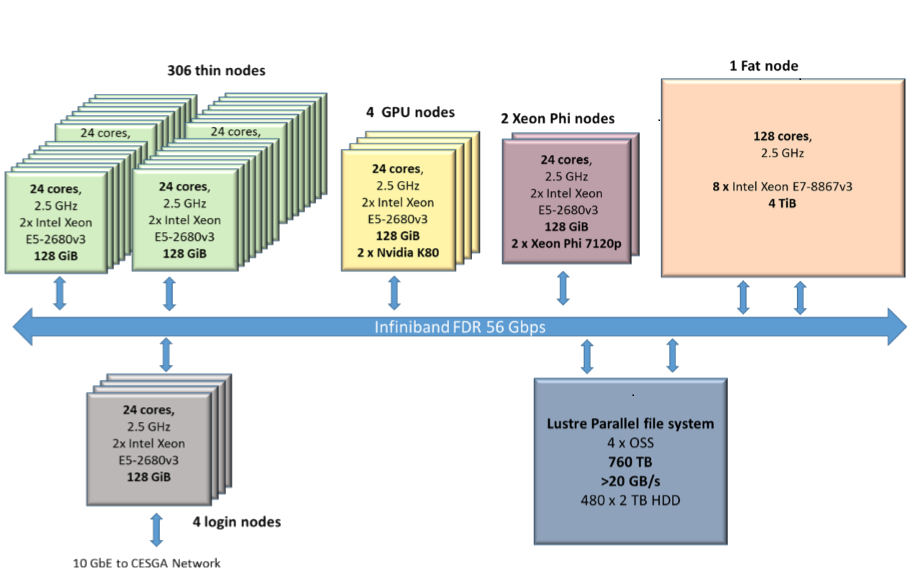
\includegraphics[width=\textwidth]{ftii}
    \caption{FT2 architecture}
  \end{figure}
}

\frame{
  \frametitle{FT2's compute nodes}

  \vspace*{-0.5cm}
  \begin{figure}
    \hspace*{-0.97cm}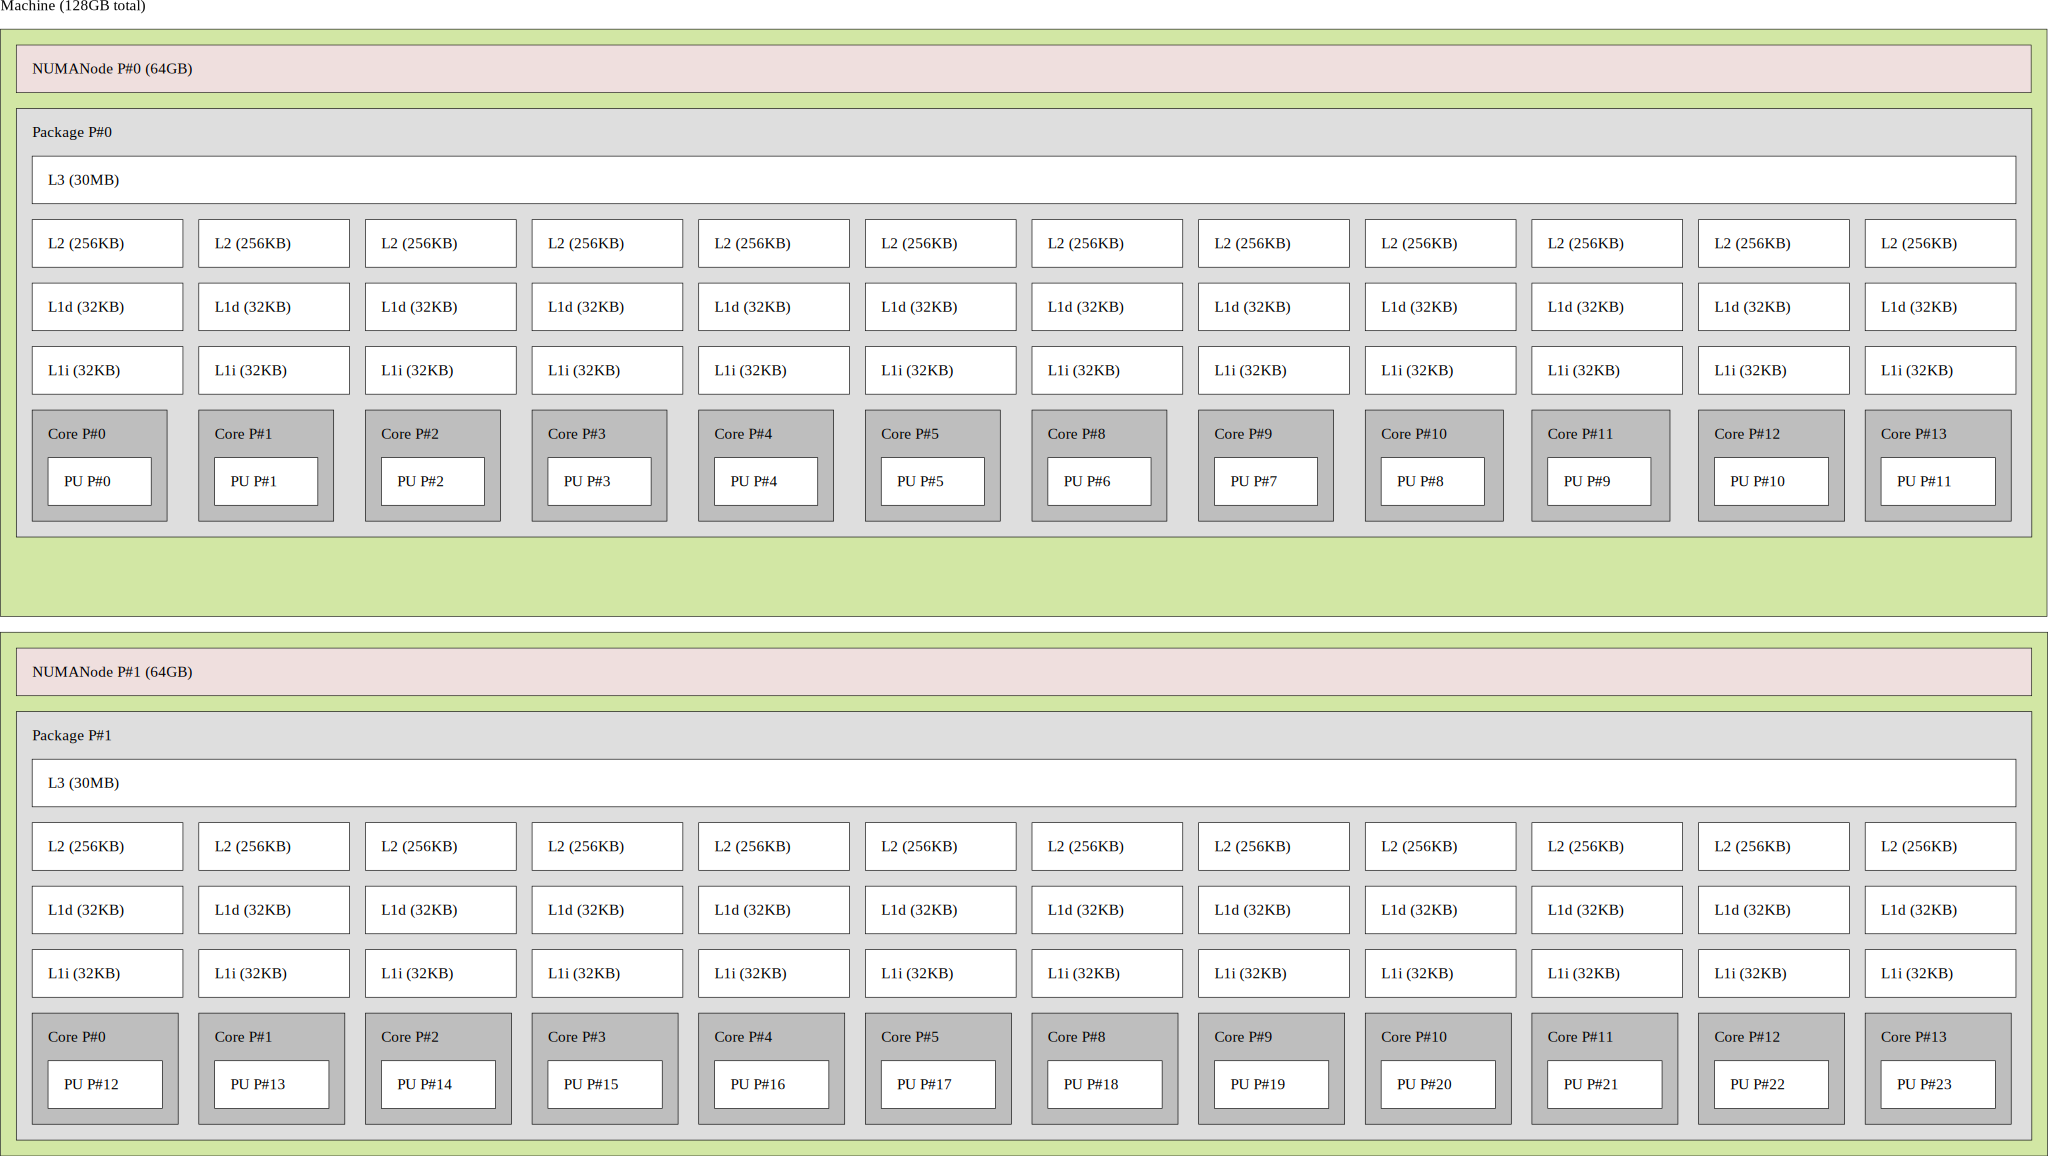
\includegraphics[width=1.18\textwidth]{ft2node}
    \caption{FT2 thin compute node}
  \end{figure}
}

\frame{
  \frametitle{Cache levels at FT2's nodes~\footnote{This and more info
    can be obtained in runtime with {\tt sysconf} (unistd.h) or with
    the command line utility {\tt getconf}}}

  \begin{description}
  \item[L1i]
    \begin{itemize}
    \item 32KB
    \item 8-way associative
    \item 64B/line
    \end{itemize}
  \item[L1d]
    \begin{itemize}
    \item 32KB
    \item 8-way associative
    \item 64B/line
    \end{itemize}
  \item[L2]
    \begin{itemize}
    \item 256KB
    \item 4-way associative
    \item 64B/line
    \end{itemize}
  \item[L3]
    \begin{itemize}
    \item 30MB
    \item 12-way associative
    \item 64B/line
    \end{itemize}
  \end{description}
}

\subsection{Performance characterization and \emph{roofline} model}

\frame{
  \frametitle{Typical performance metrics}

  \begin{itemize}
  \item CPU
    \begin{itemize}
    \item MIPS
    \item FLOPS (usually GFLOPs/sec)
    \item Computational/Arithmetic intensity: FLOP/Byte
    \end{itemize}
  \item Memory \& I/O
    \begin{itemize}
    \item Latency (time units)
    \item Bandwith/Throutput (usually GBs/sec)
    \end{itemize}
  \item Cache
    \begin{itemize}
    \item Miss/Hit rate
    \end{itemize}
  \end{itemize}
}

\frame{
  \frametitle{Performance metrics for parallel applications}

  \begin{description}
  \item[Speedup:] Measure of performance
    \begin{itemize}
    \item Ratio between sequential and parallel execution times
      $$Speedup_{nprocs} = \frac{T_{seq}}{T_{nprocs}}$$
    \end{itemize}
  \item[Efficiency] Measure of use of computational resources
    \begin{itemize}
    \item Ratio between performance and resources used to achieve it
      $$Efficiency_{nprocs} = \frac{Speedup_{nprocs}}{nprocs} =
      \frac{T_{seq}}{nprocs \times T_{nprocs}}$$
    \end{itemize}
  \end{description}
}

\frame{
  \frametitle{Parallel application's performance key: Scalability}

  \vspace*{-0.4cm}
  \begin{figure}\raggedright
    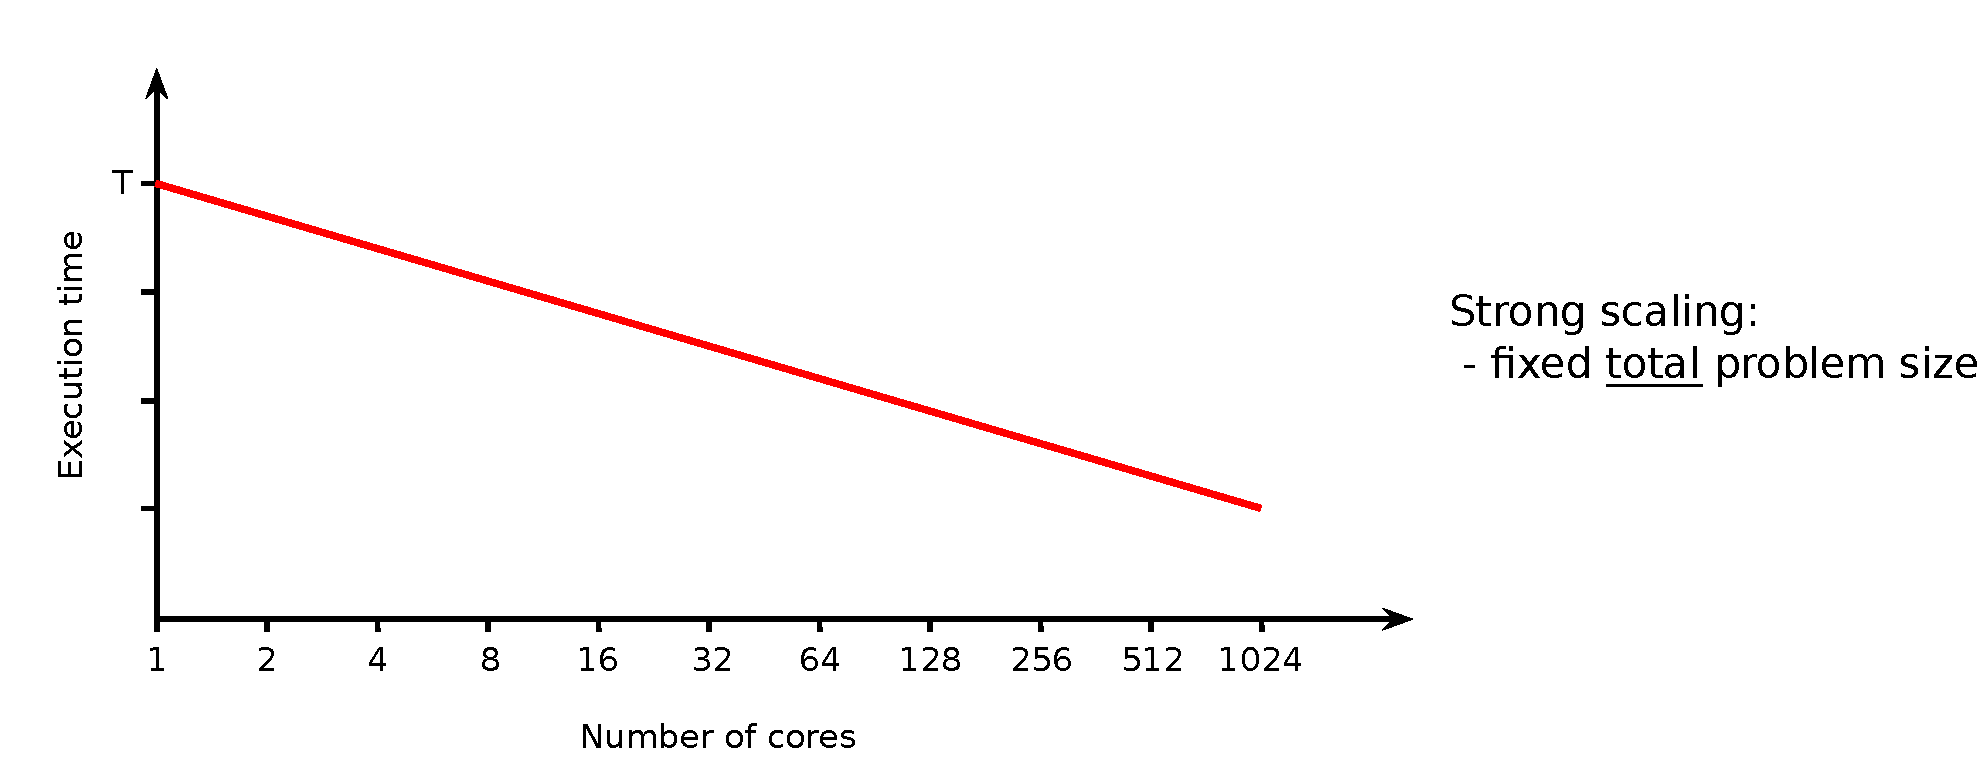
\includegraphics[height=.45\textheight]{scalability_strong}
    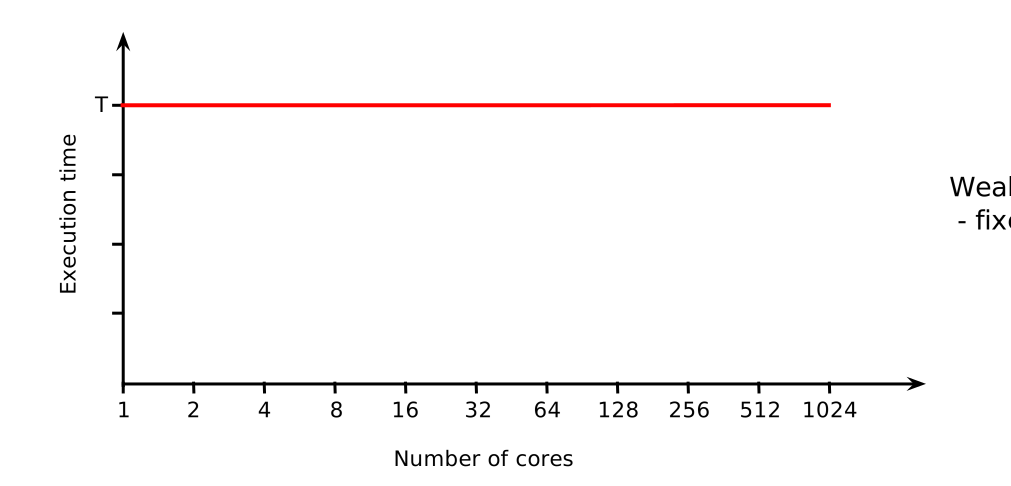
\includegraphics[height=.45\textheight]{scalability_weak}
    \caption{Scalability: {\bf weak} versus {\bf strong} scaling}
  \end{figure}
}

\frame{
  \frametitle{Performance characterization}

  Identifying the dominant bottleneck:
  \begin{itemize}
  \item Compute bound (aka CPU bound)
  \item Memory bound
    \begin{itemize}
    \item Cache bound
    \end{itemize}
  \item I/O bound
  \end{itemize}

  Obviously, in terms of velocity:
  \begin{itemize}
  \item[] CPU > Cache (L1 > L2 > L3) > Mem > I/O
  \end{itemize}

}

% Good explanation from https://stackoverflow.com/questions/868568/what-do-the-terms-cpu-bound-and-i-o-bound-mean
% CPU Bound means the rate at which process progresses is limited by the speed of the CPU. A task that performs calculations on a small set of numbers, for example multiplying small matrices, is likely to be CPU bound.

% I/O Bound means the rate at which a process progresses is limited by the speed of the I/O subsystem. A task that processes data from disk, for example, counting the number of lines in a file is likely to be I/O bound.

% Memory bound means the rate at which a process progresses is limited by the amount memory available and the speed of that memory access. A task that processes large amounts of in memory data, for example multiplying large matrices, is likely to be Memory Bound.

% Cache bound means the rate at which a process progress is limited by the amount and speed of the cache available. A task that simply processes more data than fits in the cache will be cache bound.

% I/O Bound would be slower than Memory Bound would be slower than Cache Bound would be slower than CPU Bound.

% The solution to being I/O bound isn't necessarily to get more Memory. In some situations, the access algorithm could be designed around the I/O, Memory or Cache limitations.

\frame{
  \frametitle{The Roofline Model}

  \metroset{block=fill}

  \begin{block}{Basic Roofline Model}
    Bounds Floating-point performance as a function of
    \begin{itemize}
    \item machine peak performance (GFLOPs/sec)
    \item machine peak bandwidth (GBytes/sec)
    \item arithmetic intensity (FLOPs/Byte) \hfil \alert{\small $\leftarrow$ core concept}
    \end{itemize}
  \end{block}

  \begin{figure}
    \begin{overprint}
      \onslide<1>\centering
      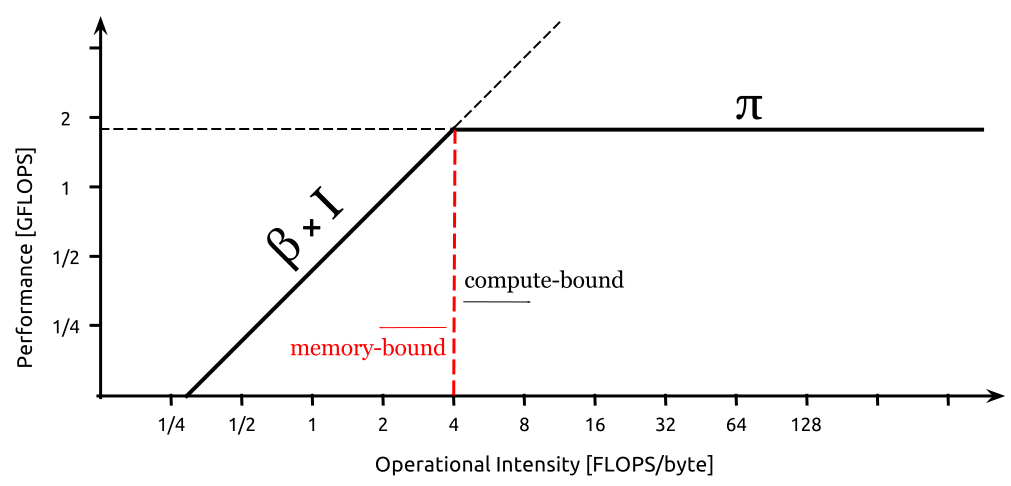
\includegraphics[width=.7\textwidth]{naive_roofline_model}
      \onslide<2>\centering
      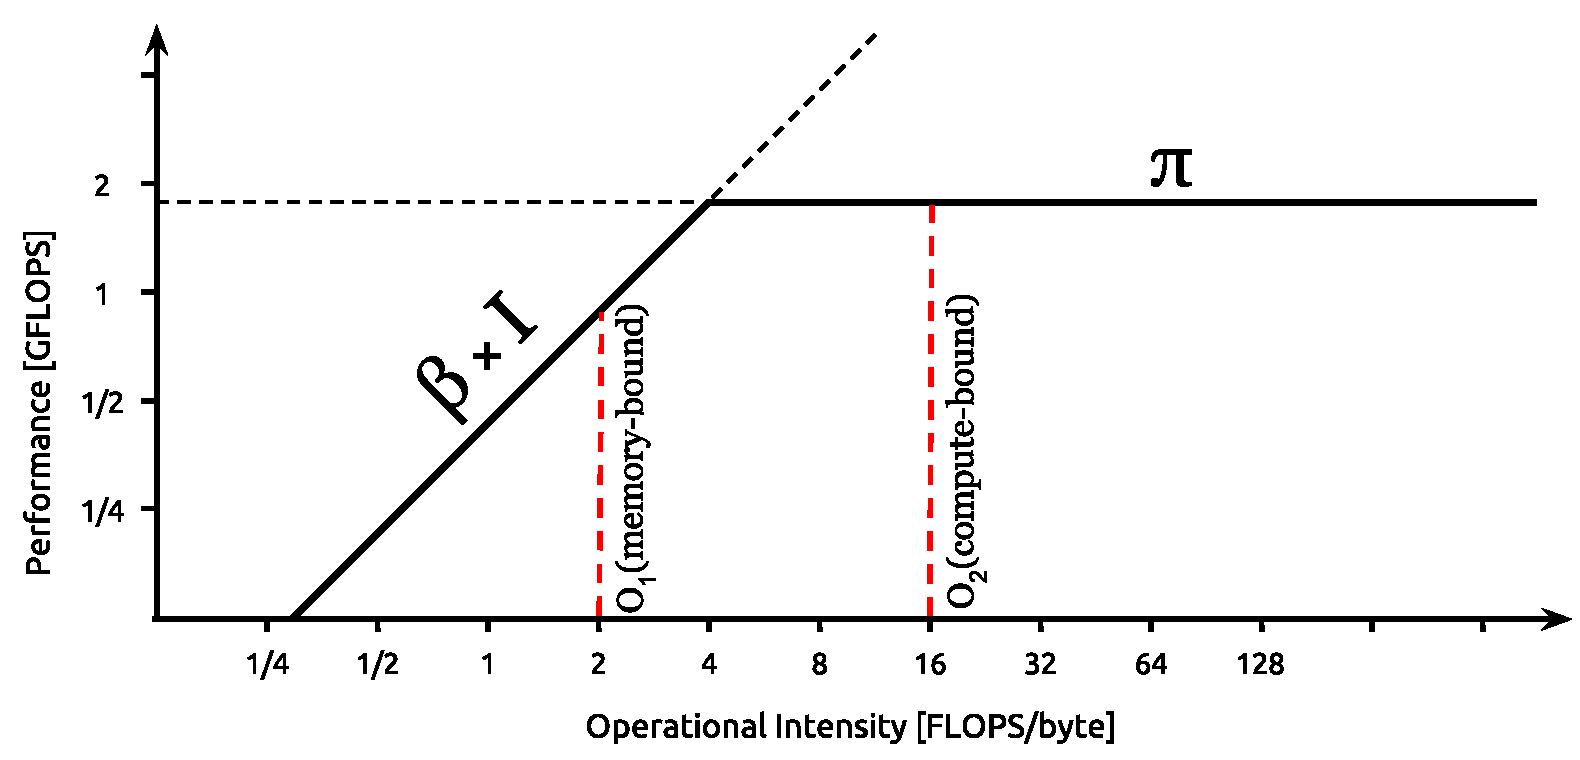
\includegraphics[width=.7\textwidth]{naive_roofline_model2}
    \end{overprint}
    \caption{Original image by Giu.natale, CC BY-SA 4.0, modified by me
      \url{https://commons.wikimedia.org/w/index.php?curid=49641351}}
  \end{figure}
}

\frame{
  \frametitle{Expanding the roofline plot}

  \begin{figure}\vspace*{-0.7cm}
    
\includegraphics[width=.5\textwidth]{roofline_model_bandwith_ceilings}~
    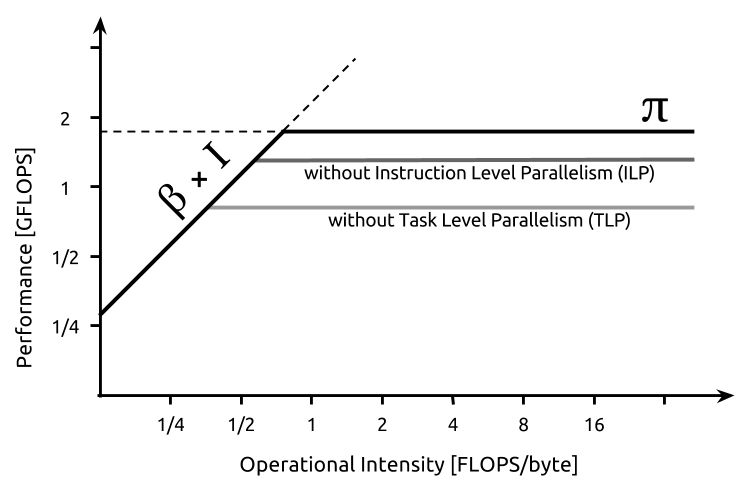
\includegraphics[width=.5\textwidth]{roofline_model_in-core_ceilings}
    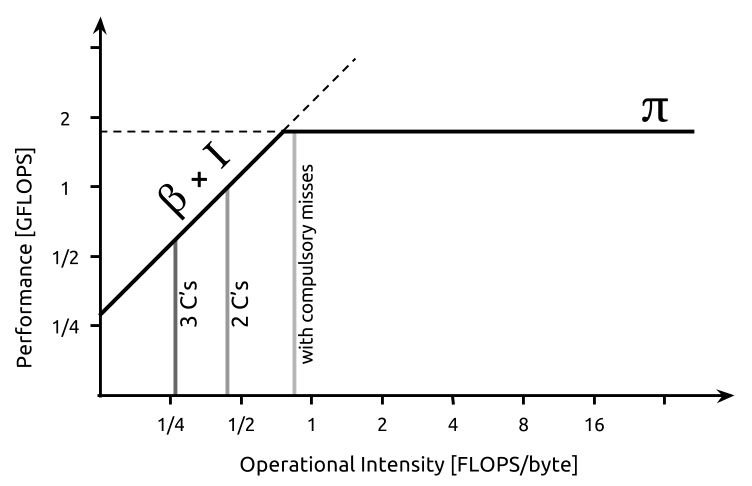
\includegraphics[width=.5\textwidth]{roofline_model_locality_walls}
    \vspace*{-0.2cm}\caption{By Giu.natale - Own work, CC BY-SA 4.0,
      \url{https://commons.wikimedia.org/w/index.php?curid=49593615}
      \url{https://commons.wikimedia.org/w/index.php?curid=49593667}
      \url{https://commons.wikimedia.org/w/index.php?curid=49593835}
    }
  \end{figure}
}

\frame{
  \frametitle{Roofline model: an intuitive visual performance model}

  \begin{itemize}
  \item Provides performance estimation
    \begin{itemize}
    \item of a given compute kernel or application
    \item on a specific platform
    \end{itemize}

    \metroset{block=fill}
    \begin{block}{Visual and intuitive: key information at a glance}
      \begin{itemize}
      \item[\checkmark] Shows inherent hardware limitations
      \item[\checkmark] Highlights potential benefit and priority of
        optimizations
      \end{itemize}
    \end{block}
  \end{itemize}

  \begin{figure}
    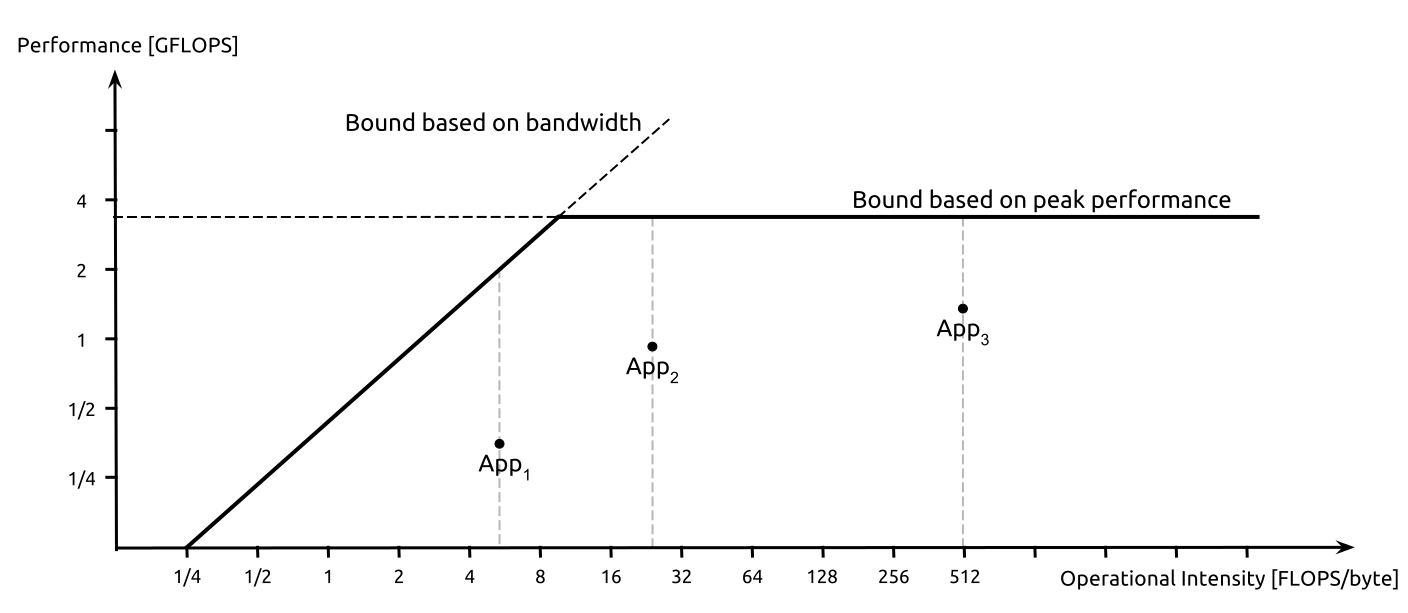
\includegraphics[width=.7\textwidth]{naive_roofline_model_example}
    \caption{By Giu.natale - Own work, CC BY-SA 4.0,
      \url{https://commons.wikimedia.org/w/index.php?curid=49641314}}
  \end{figure}
}



\section{Code optimizations at compilation time}

\frame{
  \frametitle{The art of computer programming: typical workflow}

  \begin{itemize}
  \item Coding
  \item Compiling (\& Linking)
  \item Debugging
  \item Profiling
  \item Optimizing
  \end{itemize}
}

\frame{
  \frametitle{Main tools to create efficient software}

  Main tools we'll use during this course
  \begin{description}
  \item[Compiling] ~\\
    GNU Compilers: gcc, g++, gfortran
  \item[Debugging] ~\\
    gdb
  \item[Profiling and performance analysis] ~\\
    gprof, valgrind, perf, extrae+paraver
  \item[Performance characterization] ~\\
    Berkeley Lab's CS Roofline Toolkit
  \end{description}
}

\frame{
  \frametitle{Complementary tools}

  \setbeamertemplate{itemize subsubitem}[triangle]

  \begin{itemize}
  \item A good \emph{text editor} is essential to feel comfortable
    coding/debugging/profiling/optimizing
    \begin{itemize}
    \item I like {\tt emacs} (and {\tt vim} for other purposes)
    \end{itemize}

    \pause

  \item Terminal multiplexer: {\small {\tt tmux} or {\tt screen}}

    \pause

  \item System utilities/commands:
    \begin{description}
    \item[{\small \tt top}] {\small (or {\tt htop})}
    \item[{\small \tt pstack}] ~
    \item[{\small \tt ps}] and similars\ldots
    \end{description}
    \begin{itemize}
    \item I particularly like {\tt top}:
      \begin{itemize}
      \item see load per core: {\tt 1}
      \item toggling tasks/threads: {\tt H} ({\tt -H})
      \item filtering: {\tt o} (eg. {\tt COMMAND=mybinary})
      \item field management: {\tt f} (Last used CPU\ldots)
      \end{itemize}
    \end{itemize}

    \pause

  \item Documentation and code snippets:
    \begin{itemize}
    \item {\tt man} pages (and {\tt TLDR} pages, \emph{because life is
        too short to read man pages})
    \item System documentation in {\tt /usr/share/doc}
    \item \href{https://stackoverflow.com}{
\includegraphics[width=2.5cm]{stackoverflow}}
    \end{itemize}
  \end{itemize}
}

\subsection{Understanding the compilation process}

\frame{
  \frametitle{\insertsubsectionhead: Compilers}

  \begin{quote}
    Compilers translate code from one language to another
  \end{quote}

  \pause

  \begin{description}
  \item[Source code:] usually written in a programming language
  \item[Target/Object code:] usually machine code (i.e. binary)
    \begin{itemize}
    \item[$\Rightarrow$] Most common reason: create an executable
      program
    \end{itemize}
  \end{description}
}

\frame{
  \frametitle{\insertsubsectionhead}

  \begin{figure}
    \begin{overprint}
      \onslide<1>
      \includegraphics[height=.9\textheight]{compiling}
      \onslide<2>
      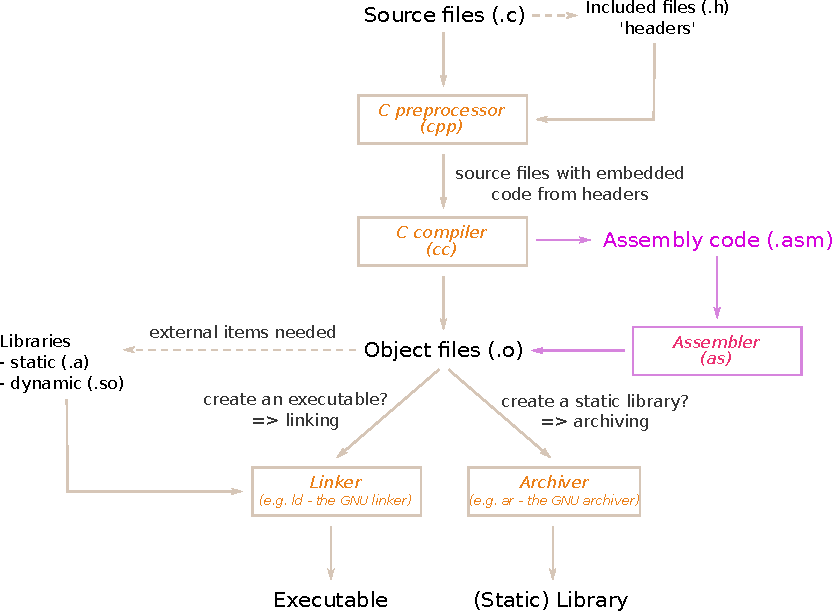
\includegraphics[height=.9\textheight]{compiling2}
    \end{overprint}
    \caption{Compilation process in C (Unix-like environments)}
  \end{figure}
}

\subsection{Operating system basics}

\frame{
  \frametitle{Processes and Threads}

  \begin{block}{\begin{quote}A process is an instance of a program
        running in the O.S.\end{quote}}

    \pause

    \begin{itemize}
    \item Each process provides the resources needed to execute a
      program:
      \begin{itemize}
      \item virtual address space, executable code, environment
        variables\ldots{} and at least one \underline{thread of
          execution}.
      \item[$\Rightarrow$] Each process is started with a single
        thread, but can create additional threads from any of its
        threads.
      \end{itemize}
    \end{itemize}
  \end{block}

  \pause

  \begin{block}{\begin{quote}A thread is an independent flow of
        control inside an address space.\end{quote}}

    \pause

    \begin{itemize}
    \item All threads of a process share its virtual address space and
      some system resources.
    \item Each threads maintains local storage and its own context:
      kernel and user stack, registers\ldots
    \end{itemize}
  \end{block}
}

\frame{
  \frametitle{Virtual Memory: Anatomy of a process in memory}

  \begin{itemize}
  \item Each process runs in its own virtual address space (kind of a
    \emph{sandbox})
  \item A portion of that virtual address space is reserved to the
    kernel
  \item The rest is user space:
  \end{itemize}

  \begin{figure}
    \includegraphics[width=0.8\textwidth]{memlayout}
    \caption{Standard segment layout in a Linux process}
  \end{figure}
}

\subsection{Basic code optimizations}

\frame{
  \frametitle{\insertsubsectionhead}

  \begin{block}{Basic code optimization techniques}
  Can be applied by
  \begin{itemize}
  \item programmer (at \emph{coding time})
  \item compiler (maybe)
  \end{itemize}
  \end{block}

  \setbeamertemplate{itemize item}[triangle]
  \begin{itemize}
  \item Loops optimizations
    \begin{itemize}
    \item Loop unrolling, Loop peeling\ldots
    \end{itemize}
  \item Inlining
  \item Reduce and improve conditionals
  \item Use registers
  \item Memory data layout
    \begin{itemize}
    \item Mem alignment, Aliasing\ldots
    \end{itemize}
  \item Prefetching
  \item Interprocedural optimizations
  \item Profile-guided optimizations (PGO)
  \item Vectorization (SIMD) and/or Parallelization (MIMD)
  \end{itemize}
}

\begin{frame}[fragile]{Basic optimization techniques: Loops (I)}

  \underline{Loop fusion}

  \begin{columns}

    \column[t]{0.45\textwidth}{
      \begin{lstlisting}[style=c,gobble=5,caption={Original code}]
        for (i=0; i<N; i++)
          x = x + a[i] + b[i];

        for (j=0; j<N; j++)
          y = y + a[i] + c[i];
      \end{lstlisting}
    }

    \column[t]{0.45\textwidth}{
      \begin{lstlisting}[style=c,gobble=5,caption={Optimized code}]
        for (i=0; i<N; i++) {
          x = x + a[i] + b[i];
          y = y + a[i] + c[i];
        }
      \end{lstlisting}
    }

  \end{columns}

\end{frame}

\begin{frame}[fragile]{Basic optimization techniques: Loops (II)}

  \underline{Loop fission} (aka loop distribution)

  \begin{columns}

    \column[t]{0.45\textwidth}{
      \begin{lstlisting}[style=c,gobble=5,caption={Original code}]
        for (i=0; i<N; i++) {
          x = x + a[i] + b[i];
          y = y + c[i] + d[i];
        }
      \end{lstlisting}
    }

    \column[t]{0.45\textwidth}{
      \begin{lstlisting}[style=c,gobble=5,caption={Optimized code}]
        for (i=0; i<N; i++)
          x = x + a[i] + b[i];

        for (i=0; i<N; i++)
          y = y + c[i] + d[i];
        }
      \end{lstlisting}
    }

  \end{columns}

\end{frame}

\begin{frame}[fragile]{Basic optimization techniques: Loops (III)}

  \underline{Loop unrolling} (aka loop unwinding)

  \begin{columns}

    \column[t]{0.45\textwidth}{
      \begin{lstlisting}[style=c,gobble=5,caption={Original code}]
        for (i=0; i<N; i++)
          x = x + a[i] + b[i];
      \end{lstlisting}
    }

    \column[t]{0.5\textwidth}{
      \begin{lstlisting}[style=c,gobble=5,caption={Optimized code}]
        for (i=0; i<N; i+=4) {
          x = x + a[i] + b[i];
          x = x + a[i+1] + b[i+1];
          x = x + a[i+2] + b[i+2];
          x = x + a[i+3] + b[i+3];
        }
      \end{lstlisting}
    }

  \end{columns}

\end{frame}

\begin{frame}[fragile]{Basic optimization techniques: Loops (IV)}

  \underline{Loop unroll-and-jam}

  \begin{columns}

    \column[t]{0.5\textwidth}{
      \begin{lstlisting}[style=c,gobble=7,caption={Original code}]
        for (i=0; i<N; i++)
          for (j=0; j<2; j++)
            x = x + a[i][j] + b[i][j];
      \end{lstlisting}
    }

    \column[t]{0.55\textwidth}{
      \begin{lstlisting}[style=c,gobble=6,caption={Optimized code}]
        for (i=0; i<N; i+=2) {
          x = x + a[i][0] + b[i][0];
          x = x + a[i][1] + b[i][1];
          x = x + a[i+1][0] + b[i+1][0];
          x = x + a[i+1][1] + b[i+1][1];
        }
      \end{lstlisting}
    }

  \end{columns}

\end{frame}

\begin{frame}[fragile]{Basic optimization techniques: Loops (V)}

  \underline{Loop interchange}

  \begin{columns}

    \column[t]{0.5\textwidth}{
      \begin{lstlisting}[style=c,gobble=7,caption={Original code}]
        for (i=0; i<N; i++)
          for (j=0; j<N; j++)
            x = x + a[j][i] + b[j][i];
      \end{lstlisting}
    }

    \column[t]{0.5\textwidth}{
      \begin{lstlisting}[style=c,gobble=7,caption={Optimized code}]
        for (j=0; j<N; j++)
          for (i=0; i<N; i++)
            x = x + a[j][i] + b[j][i];
      \end{lstlisting}
    }

  \end{columns}

\end{frame}

\begin{frame}[fragile]{Basic optimization techniques: Loops (VI)}

  \underline{Loop-invariant code motion} (aka hoisting)

  \begin{columns}

    \column[t]{0.5\textwidth}{
      \begin{lstlisting}[style=c,gobble=3,caption={Original code}]
        for (i=0; i<N; i++)
          x = x + a[i] + f(p);
      \end{lstlisting}
    }

    \column[t]{0.5\textwidth}{
      \begin{lstlisting}[style=c,gobble=3,caption={Optimized code}]
        double tmp = f(p)

        for (i=0; i<N; i++)
          x = x + a[i] + tmp;
      \end{lstlisting}
    }

  \end{columns}

\end{frame}

\begin{frame}[fragile]{Basic optimization techniques: Loops (VII)}

  \underline{Loop peeling}

  \begin{columns}

    \column[t]{0.5\textwidth}{
      \begin{lstlisting}[style=c,gobble=3,caption={Original code}]
        int p = 10;

        [...]

        for (i=0; i<N; i++) {
          x = x + a[i] + b[p];
          p = i;
        }
      \end{lstlisting}
    }

    \column[t]{0.5\textwidth}{
      \begin{lstlisting}[style=c,gobble=5,caption={Optimized code}]

        x = x + a[0] + b[10];

        for (i=0; i<N; i++)
          x = x + a[i] + b[i-1];
      \end{lstlisting}
    }

  \end{columns}

\end{frame}

\begin{frame}[fragile]{Basic optimization techniques: Loops (VIII)}

  \underline{Loop blocking / tiling}

  \begin{columns}

    \column[t]{0.4\textwidth}{
      \begin{lstlisting}[style=c,gobble=7,caption={Original code}]
        float a[10], v[1000];

        for (i=0; i<10; i++)
          for (j=0; j<1000; j++)
            a[i] += i * v[j];
      \end{lstlisting}
    }

    \column[t]{0.63\textwidth}{
      \begin{lstlisting}[style=c,gobble=7,caption={Optimized code}]
        float a[10], v[1000];

        // Let's assume 16floats/linecache
        for (jj=0; jj<1000; jj+=16)
          for (i=0; i<10; i++)
            for (j=jj; j<min(jj+16,1000); j++)
              a[i] += i * v[j];
      \end{lstlisting}
    }

  \end{columns}

\end{frame}

\begin{frame}[fragile]{Basic optimization techniques: Inlining}

  \underline{Inlining}

  \begin{columns}

    \column[t]{0.45\textwidth}{
      \begin{lstlisting}[style=c,gobble=7,caption={Original code}]
        double func(int a) {
          return sqrt(a) + sin(a);
        }

        for (i=0; i<N; i++)
          x = x + func(i);
      \end{lstlisting}
    }

    \column[t]{0.45\textwidth}{
      \begin{lstlisting}[style=c,gobble=7,caption={Optimized code}]
        for (i=0; i<N; i++)
          x = x + sqrt(i) + sin(i);
      \end{lstlisting}
    }

  \end{columns}

\end{frame}

\begin{frame}[fragile]{Basic optimization techniques: Conditionals}

  \underline{Simplify logic expressions}:
  \vspace*{-0.7cm}
  \begin{columns}

    \column[t]{0.56\textwidth}{
      \begin{lstlisting}[style=c,gobble=7,caption={Original code}]
        if (t1 == 0 && t2 == 0 && t3 == 0)
      \end{lstlisting}
    }

    \column[t]{0.4\textwidth}{
      \begin{lstlisting}[style=c,gobble=7,caption={Optimized code}]
        if ((t1 | t2 | t3) == 0)
      \end{lstlisting}
    }

  \end{columns}

  \pause

  \underline{Leverage shortcut evaluation}:
  \vspace*{-0.7cm}
  \begin{columns}

    \column[t]{0.45\textwidth}{
      \begin{lstlisting}[style=c,gobble=5,caption={Original code}]
        if (usually_true()
            && usually_false())
      \end{lstlisting}
    }

    \column[t]{0.45\textwidth}{
      \begin{lstlisting}[style=c,gobble=5,caption={Optimized code}]
        if (usually_false()
            && usually_true())
      \end{lstlisting}
    }

  \end{columns}

  \pause

  \underline{Loop-invariant conditional motion}:
  \vspace*{-1.1cm}
  \begin{columns}

    \column[t]{0.45\textwidth}{

      \begin{lstlisting}[style=c,gobble=5,caption={Original code}]
        for (i=0; i<N; i++)
          if (op == 'a')
            doOpA(v[i]);
          else if (k > 3)
            doOpB(v[i], 3);
          else
            doOpB(v[i], k);
      \end{lstlisting}
    }

    \column[t]{0.47\textwidth}{
      \begin{lstlisting}[style=c,gobble=7,caption={Optimized code}]
        if (op == 'a')
          for (i=0; i<N; i++)
            doOpA(v[i]);
        else {
          int tmp = (k > 3) ? 3 : k;
          for (i=0; i<N; i++)
            doOpB(v[i], tmp);
        }
      \end{lstlisting}
    }

  \end{columns}

\end{frame}

\subsection{Compiler optimizations}

\frame{
  \frametitle{Looking at the compiler}
  How can the compiler help us to achieve efficient binaries from our
  source codes for a specific platform?
  \begin{itemize}
  \item Optimization options

    {\small \tt gcc [-Q] --help=optimizers}

    \makebox[0pt][r]{\tiny \alert{last gcc doc $\rightarrow$}\hspace*{0.15cm}}{\scriptsize
      \url{http://gcc.gnu.org/onlinedocs/gcc/Optimize-Options.html}}

    \makebox[0pt][r]{\tiny \alert{gcc 6.4 doc $\rightarrow$}\hspace*{0.15cm}}{\scriptsize
      \url{http://gcc.gnu.org/onlinedocs/gcc-6.4.0/gcc/Optimize-Options.html}}\\[0.5cm]

  \item Target-specific / machine-dependent options (x86)

    {\tt gcc [-Q] --help=target}

    \makebox[0pt][r]{\tiny \alert{last gcc doc $\rightarrow$}\hspace*{0.15cm}}{\scriptsize
      \url{http://gcc.gnu.org/onlinedocs/gcc/x86-Options.html}}

    \makebox[0pt][r]{\tiny \alert{gcc 6.4 doc $\rightarrow$}\hspace*{0.15cm}}{\scriptsize
      \url{http://gcc.gnu.org/onlinedocs/gcc-6.4.0/gcc/x86-Options.html}}
  \end{itemize}
  }

\frame{
  \frametitle{Compiler machine-dependent options (x86)}

  (a.k.a. {\it `-m'} options)

  \begin{description}
  \item[{\tt -march={\it cpu-type}}] Generate instructions for that
    machine type\\
    E.g. {\tt native|x86-64|haswell|\ldots}
  \item[{\tt -mtune={\it cpu-type}}] Tune generated code for that
    machine type
  \item[{\tt -mavx -mavx2\ldots}] Enable the use of extended
    instruction sets (vector instructions, mostly)
  \end{description}

  \vfill
  $\rightarrow$ {\footnotesize Check target specific options with:
    {\tt gcc -Q -march=native --help=target}}
}

\frame{
  \frametitle{Compiler optimization levels}

  In a nutshell: \hfil (each level includes the previous)
  \begin{description}[{\tt -Ofast}]
  \item[{\tt -O0}] [Default] No optimization. Reduces compilation time
    and make debugging produce the expected results.
  \item[{\tt -O/-O1}] Basic optimizations. Tries to reduce code size
    and execution time, avoiding time-consuming opts.
  \item[{\tt -O2}] Optimize further, enabling opts not involving
    space-speed tradeoff. Common level for production binaries.
  \item[{\tt -O3}] Optimizes yet more. Turns on opts that can greatly
    increase code size. Due to this, sometimes is not faster than {\tt
      -O2}.
  \item[{\tt -Ofast}] Enables {\tt -ffast-math}, optimizations that
    are not valid for all standard-compliant programs.

    Additionally, Fortran-specific {\tt -fstack-arrays}, unless {\tt
      -fmax-stack-var-size} is specified, and {\tt
      -fno-protect-parens}.
  \end{description}

  $\rightarrow$ {\footnotesize Check specific options being enable/disable at
    each level for your compiler version with {\tt gcc -Q -O2
      --help=optimizers} (or in the \alert{doc})}
}

% Info about GCC's IPA:
% https://kristerw.blogspot.com/2017/05/interprocedural-optimization-in-gcc.html
\frame{
  \frametitle{Interprocedural \underline{optimization} (IPO) / \underline{analysis} (IPA)}

  \begin{itemize}
  \item Collection of compiler techniques based on analyzing the
    entire program
    \begin{itemize}
    \item[$\rightarrow$] other optimizations look at only a single function, or even a single block of code.
    \end{itemize}

  \item IPO seeks to reduce or eliminate duplicate calculations,
    inefficient use of memory, and to simplify iterative sequences
    such as loops.
    \begin{itemize}
    \item may re-order routines for better memory layout and locality
    \item may perform dead code elimination, inlining, etc.
    \end{itemize}
  \end{itemize}
}

\frame{
  \frametitle{Compiling to debug and/or profile a code}

  Compiling to {\bf debug}, basically:
  \begin{description}[{\tt -Og}]
  \item[{\tt -g}] Includes extra information to use by a debugger\\
    Typically used together with {\tt -O0} (no optimizations)
  \item[{\tt -Og}] Optimize debugging experience: enables
    optimizations that do not interfere with debugging
  \item[$\Rightarrow$] More fine tuning options in the doc

    \makebox[0pt][r]{\tiny \alert{last gcc doc $\rightarrow$}\hspace*{0.15cm}}{\scriptsize
      \url{http://gcc.gnu.org/onlinedocs/gcc/Debugging-Options.html}}

    \begingroup
    \leftskip0em
    \rightskip\leftskip
    \makebox[0pt][r]{\tiny \alert{gcc 6.4 doc $\rightarrow$}\hspace*{0.15cm}}{\scriptsize
      \url{http://gcc.gnu.org/onlinedocs/gcc-6.4.0/gcc/Debugging-Options.html}}
    \par
    \endgroup
  \end{description}

  \only<2>{
  Compiling to {\bf profile} (instrumentation options):
  \begin{description}[{\tt -pg}]
  \item[{\tt -pg}] Generate extra code to write profile information
    for {\tt gprof}\footnote{{\bf Gprof}: performance analysis tool
      for Unix applications, part of binutils \url{http://www.gnu.org/software/binutils}}
  \item[$\Rightarrow$] More fine tuning options in the doc

    \begingroup
    \leftskip0em
    \rightskip\leftskip
    \makebox[0pt][r]{\tiny \alert{last gcc doc $\rightarrow$}\hspace*{0.15cm}}{\scriptsize
      \url{http://gcc.gnu.org/onlinedocs/gcc/Instrumentation-Options.html}}
    \par
    \endgroup

    \begingroup
    \leftskip0em
    \rightskip\leftskip
    \makebox[0pt][r]{\tiny \alert{gcc 6.4 doc $\rightarrow$}\hspace*{0.15cm}}{\scriptsize
      \url{http://gcc.gnu.org/onlinedocs/gcc-6.4.0/gcc/Instrumentation-Options.html}}\\
    ~
    \par
    \endgroup
  \end{description}
  }
}

\begin{frame}[fragile]{Other interesting compiler options}

  \begin{itemize}
  \item I like to activate all relevant \emph{warnings}: {\tt -Wall
      -Wextra}
  \item Use {\tt -D} to pass macros used in the code to precompiler

    \pause

  \item Generate ASM code \emph{``easy to read''} (e.g. to check
    vectorization)
        \begin{lstlisting}[style=shell,gobble=5,caption={From the book
\emph{Algorithms for programmers}\footnote<2>{Algorithms for programmers:
\url{https://www.jjj.de/fxt}}\footnote<2>{Generating Mixed
Source and Assembly List using GCC: {\scriptsize \url{http://www.systutorials.com/240/generate-a-mixed-source-and-assembly-listing-using-gcc}}}}]
         # create assembler code:
         cc -S -fverbose-asm -g -O2 test.cc -o test.s

         # create asm interlaced with source lines:
         as -alhnd test.s > test.lst
       \end{lstlisting}
  \end{itemize}

\end{frame}


\section{Helping the compiler to optimize}

\frame{
  \frametitle{Some key optimizations at compilation/coding
    time~\footnote{This slide is replicated on purpose!}}

    Can be applied by
    \begin{itemize}
    \item programmer (at \emph{coding time})
    \item compiler (maybe)
    \end{itemize}

  \setbeamertemplate{itemize item}[triangle]
  \begin{itemize}
  \item Loops optimizations
    \begin{itemize}
    \item Loop unrolling, Loop peeling\ldots
    \end{itemize}
  \item Inlining
  \item Reduce and improve conditionals
  \item Use registers
  \item Memory data layout
    \begin{itemize}
    \item Mem alignment, Aliasing\ldots
    \end{itemize}
  \item Prefetching
  \item Interprocedural optimizations
  \item Profile-guided optimizations (PGO)
  \item Vectorization (SIMD) and/or Parallelization (MIMD)
  \end{itemize}
}

\begin{frame}[fragile]{Helping the compiler to optimize code}

  \begin{itemize}
  \item Declaring {\bf attributes}: \hfil {\tt \_\_attribute\_\_(( ))}
    \begin{itemize}
    \item of functions~\footnote{\url{http://gcc.gnu.org/onlinedocs/gcc/Function-Attributes.html}}
    \item of variables~\footnote{\url{http://gcc.gnu.org/onlinedocs/gcc/Variable-Attributes.html}}
    \item of types~\footnote{\url{http://gcc.gnu.org/onlinedocs/gcc/Type-Attributes.html}}
    \item etc.
    \end{itemize}
  \end{itemize}

  \begin{lstlisting}[style=c,gobble=2,caption={Example: assume an
      aligned pointer is returned}]
    void* my_alloc1(size_t) __attribute__((assume_aligned(16)))
  \end{lstlisting}

  \pause

  \begin{itemize}
  \item Let's notice: There is some overlap between the purposes of
    \underline{attributes} and \underline{pragmas}
  \item Even though {\tt gcc} recommends {\tt \_\_attribute\_\_}, it
    keeps {\tt \#pragma} mainly for compatibility issues
  \end{itemize}


\end{frame}

\begin{frame}[fragile]{Helping the compiler to optimize code}

  \begin{itemize}
  \item Prefetch: {\footnotesize \tt \_\_builtin\_prefetch (const void
      *addr, ...)}
    \begin{itemize}
    \item use it carefully\ldots
    \end{itemize}

    \begin{lstlisting}[style=c,gobble=2,caption={Prefetching example}]
      for (i = 0; i < n; i++) {
        a[i] = a[i] + b[i];
        __builtin_prefetch (&a[i+j], 1, 1);
        __builtin_prefetch (&b[i+j], 0, 1);

        /* … */
      }
    \end{lstlisting}
  \end{itemize}

\end{frame}


\frame{
  \frametitle{Profile-guided optimization (PGO)}

  \begin{enumerate}
  \item {\bf First compilation phase}: Instrument the application with profiling code
    \begin{itemize}
    \item[$\rightarrow$] application will log profiling data when running
    \end{itemize}
  \item {\bf Execute the instrumented binary}
    \begin{itemize}
    \item[$\rightarrow$] profiling files are generated for each run
    \end{itemize}
  \item {\bf Second compilation phase}: Rebuild the application to
    leverage profiling data to optimize it
  \end{enumerate}
}

\frame{
  \frametitle{Profile-guided optimization (PGO) in gcc}

  \begin{description}
  \item[{\tt -fprofile-generate}] enables \begin{itemize}
    \item[] {\tt -fprofile-arcs}
    \item[] {\tt -fprofile-values}
    \item[] {\tt -fvpt}
    \end{itemize}
  \end{description}
  \begin{enumerate}
  \item A {\tt .gcno} file is generated for each object file
    \begin{itemize}
    \item these files are also used for {\tt gcov} coverage reports
    \end{itemize}
  \item Then, multiple executions record coverage data into .gcda
    files
  \item Finally, recompile with {\tt -fprofile-use}
    \begin{itemize}
    \item gathers the coverage data and infer if a branch is
      likely/unlikely
    \end{itemize}
  \item[$\rightarrow$] Resulting binary will be better at prefetching code
  \end{enumerate}
  \begin{description}
  \item[{\tt -fprofile-use}] enables \begin{itemize}
    \item[] {\tt -fbranch-probabilities}
    \item[] {\tt -fvpt}
    \item[] {\tt -funroll-loops}
    \item[] {\tt -fpeel-loops}
    \item[] {\tt -ftracer}
    \end{itemize}
  \end{description}
}


\subsection{Auto-vectorization}

\begin{frame}[fragile]{Vectorization}

  \begin{description}
  \item[Vectorization] Form of SIMD which allows us to crunch multiple
    values in one CPU instruction
  \end{description}

  $\Rightarrow$ Especially useful to \underline{optimize loop execution} (but not
  exclusively)

  \begin{columns}
    \column{0.45\textwidth}{
      \begin{lstlisting}[style=c,gobble=7,caption={Sequential loop}]
        float A[32], B[32], C[32];

        for (i=0; i<32; i++)
          C[i] = A[i] + B[i];
          // 32 float ADD ops
      \end{lstlisting}
    } \
    \column{0.55\textwidth}{
      \begin{lstlisting}[style=c,gobble=7,caption={Vectorized pseudocode}]
        float A[32], B[32], C[32];

        for (i=0; i<32; i+=8)
          C[i:i+7] = A[i:i+7] + B[i:i+7];
          // vectorization factor: 8
          // => 4 vector float ADD ops
      \end{lstlisting}
    }
  \end{columns}
\end{frame}

\frame{
  \frametitle{Vectorization: Intel SIMD extensions}

  \begin{figure}
    \includegraphics{avx_regs}
    \caption{x86-64 Vector Registers}
  \end{figure}
  \begin{itemize}
  \item AVX-512 (ZMM0--ZMM31)
  \item AVX/AVX2 (YMM0--YMM31) \quad \alert{\small $\rightarrow$ AVX2 in FT2's Haswell procs}
  \item SSE (XMM0--XMM31)
  \end{itemize}
}

\begin{frame}[fragile]{Vectorization: x86-64 vector operations}

  \begin{itemize}
  \item Intrinsic C-like functions to access vector instructions\\
    e.g.\\[0.2cm]
    \begin{columns}
      \column{0.33\textwidth}{
        {\bf AVX asm instruction}\\[-0.5cm]
        \begin{lstlisting}[style=asm,gobble=8]
          vmovaps ymm, m256
        \end{lstlisting}
      } \
      \column{0.77\textwidth}{
        {\bf Intrinsic function}\\[-0.5cm]
        \begin{lstlisting}[style=c,gobble=8]
          __m256 _mm256_load_ps (float const *mem_addr)
          #include <immintrin.h>
        \end{lstlisting}
      }
    \end{columns}

  \item[] \hspace*{-0.7cm} \mbox{\scriptsize \alert{(doc)} Intrinsics Guide: \url{http://software.intel.com/sites/landingpage/IntrinsicsGuide}}\\[0.2cm]
  \item SIMD instructions typically require:
    \begin{itemize}
    \item aligned data {\footnotesize (although there are slower {\tt
          load} and {\tt store} operations for unaligned data)}
    \item no pointer aliasing {\footnotesize (pointers are aliased if they can refer to same storage location)}
    \end{itemize}
  \end{itemize}

  \pause

  \begin{columns}
    \column{0.35\textwidth}{
      \begin{alertblock}{Writing vectorized code}
        \begin{itemize}
        \item hard
        \item error-prone
        \end{itemize}
      \end{alertblock}
    }
    \column{0.01\textwidth}{
      \mbox{$\Rightarrow$}
    }
    \column{0.5\textwidth}{
      \begin{exampleblock}{Autovectorization}
        \structure{\checkmark} Let compiler do it for you\\
        \pause
        {\small $\rightarrow$ Sometimes, compiler needs some help, though}
      \end{exampleblock}
    }
  \end{columns}
\end{frame}

\frame{
  \frametitle{Vectorization: requirements and limitations}

  \textcolor{green}{ Which kind of loops can be vectorized?}
  \begin{itemize}
  \item Countable loops: The number of iterations has to be known at run-time
  \item The loop has to have single entry and exit points {\small (e.g. We cannot have a break statement inside the loop)}
  \item Conditional statements are allowed in a loop if they can be replaced by masks
  \item No function calls
    \begin{itemize}
    \item Except vectorizable math functions e.g. {\tt sin}, {\tt sqrt},\ldots
    \end{itemize}
  \item Loop to be vectorized must be innermost loop if nested
  \end{itemize}
}

\begin{frame}[fragile]{Vectorization: requirements and limitations}

  \textcolor{red}{Obstacles to vectorization}
  \begin{itemize}
  \item Non-contiguous memory access patterns
  \item Loop-carried dependences\footnote{Data dependency: \url{https://en.wikipedia.org/wiki/Data_dependency}}
    \begin{description}
    \item[\underline{RAW} (Read After Write)] ~\\
      \begin{minipage}{5cm}
        \begin{lstlisting}[style=c,gobble=4,caption={\bf \textcolor{red}{The loop cannot be vectorized}}]
          for (i=0; i<N; i++)
            a[i] = a[i-1] + 1;
        \end{lstlisting}
      \end{minipage}

      \vspace*{0.5cm}

    \item[\underline{WAR} (Write after Read)] ~\\
      \begin{columns}
        \column{0.45\textwidth}{
          \begin{lstlisting}[style=c,gobble=7,caption={\bf \textcolor{green}{It can be vectorized}}]
            for (i=0; i<N; i++)
              a[i] = a[i+1] + 1;
          \end{lstlisting}
        } \
        \column{0.45\textwidth}{
          \begin{lstlisting}[style=c,gobble=7,caption={\bf \textcolor{red}{It cannot be vectorized}}]
            for(i=0; i<N; i++) {
              a[i] = a[i+1] + 1;
              b[i] = a[i] * 2;
            }
          \end{lstlisting}
        }
      \end{columns}
    \end{description}
  \end{itemize}

\end{frame}

\begin{frame}[fragile]{Vectorization: requirements and limitations}

  \begin{description}
  \item[\underline{WAW} (Write after Write)] ~\\
    \begin{columns}
      \column{0.45\textwidth}{
        {\bf \textcolor{red}{In general it cannnot be vectorized}}\\
      } \
      \column{0.45\textwidth}{
        {\bf \textcolor{green}{It can be vectorized} because it can be recognized by the compiler as a sum reduction}\\
        \begin{lstlisting}[style=c,gobble=6]
          for (i=0; i<N; i++)
            sum = sum + a[i];
        \end{lstlisting}
      }
    \end{columns}

  \item[\underline{RAR} (Read after Read)] The loop can be vectorized
  \end{description}
\end{frame}

\begin{frame}[fragile]{Favour autovectorization}

  \begin{itemize}
  \item Use (normally 32-bytes) aligned data structures
    \begin{itemize}
    \item There are special vector {\tt load} and {\tt store} instructions for unaligned data {\small (but they are much slower)}
    \item Use a Structure of Arrays (SoA)
      \begin{lstlisting}[style=c]
        typedef struct {
          double a[N];
          double b[N];
          double c[N];
        } mysoa;
      \end{lstlisting}
    \item instead of an Array of Structures (AoS)
      \begin{lstlisting}[style=c]
        typedef struct {
          double a,b,c;
        } aos;

        aos myaos[N];
      \end{lstlisting}
    \end{itemize}
  \end{itemize}

\end{frame}

\begin{frame}[fragile]{Favour autovectorization}

  \begin{itemize}
  \item Use data format of the minimum possible size {\small (e.g. floats instead of doubles, if possible)}
  \item Don't mix different vectorizable data types in a loop, if possible {\small (e.g. floats and doubles)}
  \item Use the {\tt restrict}~\footnote{\url{http://en.wikipedia.org/wiki/Restrict}} qualifier in the declaration of a pointer to assert there is not aliasing {\small (two pointers pointing to the same memory location)}
  \end{itemize}

\end{frame}

\frame{
  \frametitle{GCC autovectorization compiler flags}

  \begin{description}
  \item[{\tt -ftree-loop-vectorize}] Enable loop vectorization
  \item[{\tt -ftree-slp-vectorize}] Enable basic block vectorization (SLP)
  \end{description}
  \begin{itemize}
  \item Both flags are enabled by default in {\tt -O3} and {\tt
      -Ofast}, and are also enabled with {\tt -ftree-vectorize}
  \item {\tt Ofast}'s additional (unsafe) math optims may help autovect
  \item Do not forget {\tt -march=native}
  \item Reports: list (not) vectorized loops + extra info
    {\tt -fopt-info-vec}\\
    {\tt -fopt-info-vec-missed}\\
    {\tt -fopt-info-vec-all} {\footnotesize(detailed autovect process)}
  % \item Additionally:
  %   \begin{description}
  %   \item[{\tt -fvect-cost-model=[unlimited|dynamic|cheap]}] Specifies
  %     the cost model for vectorization
  %     %(default O3/Ofast: {\tt dynamic})
  %   \item[{\tt -fsimd-cost-model=[unlimited|dynamic|cheap]}] Specifies
  %     the vectorization cost model for code marked with a simd
  %     directive
  %     %(default O3/Ofast: {\tt unlimited})
  % \end{description}
  \end{itemize}
}

\frame{
  \frametitle{GCC autovectorization: compiler directives and C keywords}

  GCC Vectorization
  pragmas~\footnote{\url{http://gcc.gnu.org/onlinedocs/gcc/Loop-Specific-Pragmas.html}}:
  \begin{itemize}
  \item {\tt \#pragma GCC ivdep}
    \begin{itemize}
    \item programmer asserts no loop-carried dependencies
    \end{itemize}
  \item {\tt \#pragma omp simd [clause [,clause ]\ldots]}
    \begin{itemize}
    \item the loop can be transformed into a SIMD loop $\Rightarrow$ vectorized!
    \end{itemize}
  \end{itemize}

  C keywords:
  \begin{itemize}
  \item {\tt restrict}~\footnote{\url{http://en.wikipedia.org/wiki/Restrict}}
    \begin{itemize}
    \item used in pointer declarations to assert there's no aliasing
    \end{itemize}
  \end{itemize}
}

% \frame{
%   \frametitle{Vectorization: requirements and limitations}

%   \begin{itemize}
%   \item Countable loops
%   \item No backward loop-carried dependencies
%   \item No function calls
%     \begin{itemize}
%     \item Except vectorizable math functions e.g. sin, sqrt,\ldots
%     \end{itemize}
%   \item Straight-line code (only one control flow: no switch)
%   \item Loop to be vectorized must be innermost loop if nested
%   \end{itemize}
% }


\subsection{Auto-parallelization}

% Autopar in gcc
% Reference: https://gcc.gnu.org/wiki/AutoParInGCC
% Reference: https://gcc.gnu.org/wiki/Graphite/Parallelization
\frame{
  \frametitle{Automatic Parallelization}

  Two flags are needed:
  \begin{description}
  \item[\tt -floop-parallelize-all] Triggers the first compiler pass
    to mark loops that can be parallel
  \item[\tt -ftree-parallelize-loops=<nthreads>] Triggers the code
    generation part with the desired multi-threading level
    \begin{itemize}
    \item[$\rightarrow$] implies {\tt -pthread}
    \end{itemize}
  \end{description}
}


\section{Profiling of applications}

\frame{
  \frametitle{Profile first, optimize later}

  \begin{quote}
    Premature optimization is the root of all evil -- {Donald Knuth}
  \end{quote}
}

\frame{
  \frametitle{Profiling}

  \metroset{block=fill}
  \begin{block}{Why to profile?}
    \begin{itemize}
    \item Evaluate performance
    \item Find the performance bottlenecks
      \begin{itemize}
      \item inefficient programming / bugs
      \item memory and I/O bottlenecks
      \item parallel scaling
      \end{itemize}
    \end{itemize}
  \end{block}

  \begin{itemize}
  \item Profiling tools help you analyze your code's performance:
    \begin{itemize}
    \item how often each line of code executes
    \item what lines of code are actually executed
    \item how much computing time each section of code uses
    \item load balancing and idle periods in parallel executions
    \end{itemize}
  \end{itemize}
}

\frame{
  \frametitle{Types of profiling}

  \begin{block}{Typical profiling tasks:}
    \begin{itemize}
    \item Time-based profiling (\emph{Wall time})
    \item Memory profiling
    \item Cache profiling
    \item I/O profiling\ldots
    \end{itemize}
  \end{block}

  \pause

  \begin{block}{2 main approaches:}
    \begin{itemize}
    \item Instrumenting profiler
      \begin{itemize}
      \item automatic instrumentation
        \begin{itemize}
        \item at compiling/linking time or on the fly
        \end{itemize}
      \item user-guided instrumentation
      \end{itemize}
    \item Sampling profiler
      \begin{itemize}
      \item hardware counters
      \item system information
      \end{itemize}
    \end{itemize}
  \end{block}
}



\subsection{Execution time-based profiling: detecting bottlenecks/hot spots}

\begin{frame}[fragile]{First approach: self-profiling!}

  \begin{itemize}
  \item Naive way of measuring tasks' execution time:
    \begin{itemize}
    \item {\tt time} shell built-in command
    \item {\tt time} utility (usually in {\tt /usr/bin/time})
    \end{itemize}

    \pause

  \item Insert explicit \emph{timestamps} in your code
    \begin{itemize}
    \item DIY instrumentation: useful when you're writing your own code
      \begin{itemize}
      \item you know the structure/flow $\Rightarrow$ where to measure
      \end{itemize}
    \end{itemize}

    \pause

  \item In C, I like the function {\tt gettimeofday()}
    \begin{itemize}
    \item wall-clock time with microseconds precision ({\it hardware
        dependent})
    \end{itemize}
  \end{itemize}

  \vspace*{-0.35cm}
  \begin{overprint}
    \onslide<3>
    \begin{lstlisting}[style=c,gobble=3]
      #include <sys/time.h>

      int gettimeofday(struct timeval *tv, struct timezone *tz);
    \end{lstlisting}
    \vspace*{-0.2cm}
    \begin{lstlisting}[style=c,gobble=3]
      struct timeval {
        time_t      tv_sec;   /* seconds */
        suseconds_t tv_usec;  /* microseconds */
      };
      struct timezone {
        int tz_minuteswest;   /* minutes west of Greenwich */
        int tz_dsttime;       /* type of DST correction */
      };
    \end{lstlisting}

    \onslide<4>
    \begin{itemize}
    \item Other good options:
      \begin{description}[{\tt clock\_gettime}]
      \item[{\tt clock\_gettime}]
      \item[{\tt clock}]
      \item[{\tt time}]
        \begin{itemize}
        \item both from {\tt \#include <time.h>}
        \item also wall-clock time\\[0.2cm]
        \end{itemize}
      \item[{\tt getrusage}]
        \begin{itemize}
        \item {\tt \#include <sys/time.h>}\\
          {\tt \#include <sys/resource.h>}
        \item \emph{user} and \emph{system} times separately
        \end{itemize}

      \end{description}
    \end{itemize}
  \end{overprint}
\end{frame}

\frame{
  \frametitle{GPROF: the GNU Profiler}

  \begin{overprint}
    {\bf Gprof}: performance analysis tool for Unix applications, part of
    binutils\footnote{\url{http://www.gnu.org/software/binutils}}
    \begin{itemize}
    \item hybrid (compiler assisted) \emph{instrument.} and
      \emph{sampling} approach
    \end{itemize}

    How to use it:
    \begin{enumerate}
    \item Have profiling enabled while compiling the code
      \uncover<2->{
        \begin{itemize}
        \item[$\rightarrow$] gcc profiling flag: {\tt -pg}
        \end{itemize}
      }
    \item Execute the program code to produce the profiling data
      \uncover<2->{
        \begin{itemize}
        \item[$\rightarrow$] {\tt gmon.out} archive is generated
        \end{itemize}
      }
    \item Run the gprof tool on the profiling data file (generated in
      the step above)
      \uncover<2->{
        \begin{itemize}
        \item[{\tt \$}] {\tt gprof program\_binary [gmon.out]}
        \end{itemize}
      }
    \end{enumerate}

    \onslide<3>
    \vfill
    What GPROF provides:
    \begin{itemize}
    \item Flat profile
    \item Call graph
    \end{itemize}
    \quad
  \end{overprint}
}

\begin{frame}[fragile]{GPROF: Flat profile}

  \begin{block}{Flat Profile}
    \begin{itemize}
    \item Time spent executing each function {\small (sampled
        $\Rightarrow$ statistical inac.)}
    \end{itemize}
  \end{block}

  \begin{lstlisting}[gobble=3, caption={Flat profile example}]
    Each sample counts as 0.01 seconds.
      %   cumulative   self              self     total
     time   seconds   seconds    calls  ms/call  ms/call  name
     33.34      0.02     0.02     7208     0.00     0.00  open
     16.67      0.03     0.01      244     0.04     0.12  offtime
     16.67      0.04     0.01        8     1.25     1.25  memccpy
     16.67      0.05     0.01        7     1.43     1.43  write
     16.67      0.06     0.01                             mcount
      0.00      0.06     0.00      236     0.00     0.00  tzset
      0.00      0.06     0.00      192     0.00     0.00  tolower
      0.00      0.06     0.00       47     0.00     0.00  strlen
      0.00      0.06     0.00       45     0.00     0.00  strchr
      0.00      0.06     0.00        1     0.00    50.00  main
      0.00      0.06     0.00        1     0.00     0.00  memcpy
      0.00      0.06     0.00        1     0.00    10.11  print
      ...
  \end{lstlisting}

\end{frame}

\begin{frame}[fragile]{GPROF: Call graph}

  \begin{block}{ Call Graph}
    \begin{itemize}
    \item Time spent in each function and its children
    \end{itemize}
  \end{block}

  \begin{lstlisting}[gobble=3, basicstyle=\scriptsize\ttfamily, caption={Call graph example}]
    granularity: each sample hit covers 2 byte(s) for 20.00% of 0.05 seconds

    index % time    self  children    called     name
                                                     <spontaneous>
    [1]    100.0    0.00    0.05                 start [1]
                    0.00    0.05       1/1           main [2]
                    0.00    0.00       1/2           on_exit [28]
                    0.00    0.00       1/1           exit [59]
    -----------------------------------------------
                    0.00    0.05       1/1           start [1]
    [2]    100.0    0.00    0.05       1         main [2]
                    0.00    0.05       1/1           report [3]
    -----------------------------------------------
                    0.00    0.05       1/1           main [2]
    [3]    100.0    0.00    0.05       1         report [3]
                    0.00    0.03       8/8           timelocal [6]
                    0.00    0.01       1/1           print [9]
                    0.00    0.01       9/9           fgets [12]
                    0.00    0.00      12/34          strncmp <cycle 1> [40]
                    0.00    0.00       8/8           lookup [20]
                    0.00    0.00       1/1           fopen [21]
                    0.00    0.00       8/8           chewtime [24]
                    0.00    0.00       8/16          skipspace [44]
    -----------------------------------------------
    [4]     59.8    0.01        0.02       8+472     <cycle 2 as a whole> [4]
                    0.01        0.02     244+260         offtime <cycle 2> [7]
                    0.00        0.00     236+1           tzset <cycle 2> [26]
    -----------------------------------------------
  \end{lstlisting}
\end{frame}

\frame{
  \frametitle{GPROF: profiling options}

  Some useful parameters:
  \begin{description}
  \item[{\tt -s}] combine the data from several runs to minimize
    statistical inaccuracy in measures
  \item[{\tt -a}] suppress the printing of statically declared
    (private) functions
  \item[{\tt -b}] suppress verbose blurbs
  \item[{\tt -pfunct\_name}] flat profile for a specific function
  \item[{\tt -qfunct\_name}] call graph for a specific function
  \end{description}
}

\begin{frame}[fragile]{Obtaining a visual output: {\tt Gprof} and {\tt
      gprof2dot}}

  \begin{block}{gprof2dot}
    Python script to convert output from many profilers into a dot graph
  \end{block}

  \begin{lstlisting}[gobble=3]
    gprof program\_binary [gmon.out] | gprof2dot.py \
                                     | dot -Tpng -o output.png
  \end{lstlisting}

  \begin{figure}
    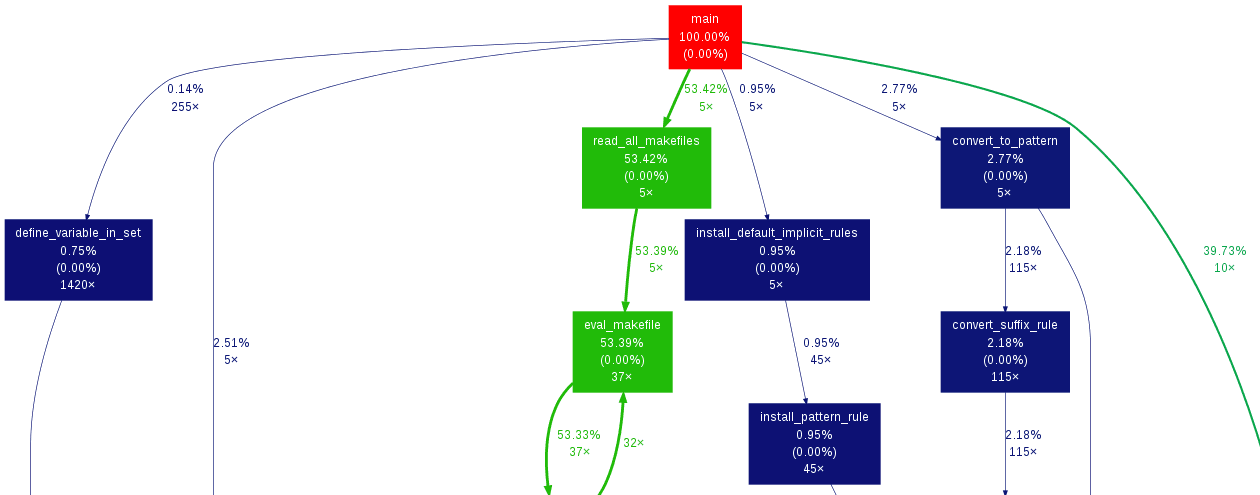
\includegraphics{gprof2dot_ex}
  \end{figure}

  \begin{columns}
    \column{.45\textwidth}{
      \begin{exampleblock}{Requirements}
        $\text{Python2} \geq 2.7$ or $\text{Python3} \geq 3.3$\\
        Graphviz
      \end{exampleblock}
    }
    \column{.6\textwidth}{
      \begin{alertblock}{Source \& pip package}
        {\footnotesize \url{http://github.com/jrfonseca/gprof2dot}}\\
        {\footnotesize \tt \$~pip install gprof2dot}
      \end{alertblock}
    }
  \end{columns}
\end{frame}

\frame{
  \frametitle{Gprof: caveats}

  GPROF main drawbacks:
  \begin{itemize}
  \item Relatively high overhead (mainly caused by instrumentation)
  \item Does not support profiling multi-threaded applications!
    \begin{itemize}
    \item there are some workarounds\ldots~\footnote{\mbox{gprof \& multithreaded code: {\scriptsize
      \url{http://sam.zoy.org/writings/programming/gprof.html}}}
  }~\footnote{gprof
        \& MPI: {\scriptsize \url{http://shwina.github.io/2014/11/profiling-parallel}}}
    \end{itemize}
  \item Cannot profile shared libraries
  \item Blind to I/O
  \item Other unexpected/weird behaviors
  \end{itemize}
}

\frame{
  \frametitle{Valgrind: a swiss army knife tool}

  {\bf Valgrind~\footnote{\url{http://valgrind.org}}:} instrumentation \underline{framework} for building
  analysis tools
  \begin{itemize}
  \item
    Cross-platform~\footnote{\url{http://valgrind.org/info/platforms.html}}
  \item Typical use:
    \begin{itemize}
    \item debugging: detect memory management and threading bugs
    \item profiling: cache, mem, branches\ldots
    \end{itemize}
  \item ... but you can also use Valgrind to build your own tool!
  \end{itemize}

  \begin{block}{Valgrind is basically a virtual machine}
  \begin{itemize}
  \item[$\rightarrow$] just in time recompilation of x86 machine code
    to some simpler RISC-like intermediate code: UCode
  \item[$\rightarrow$] depending on the chosen tool, UCode is instrumented appropriately to record the data of interest
  \end{itemize}
  \end{block}
}

\frame{
  \frametitle{Valgrind: tools provided}

  6 tools included in current versions:
  \begin{description}
  \item[Memcheck:] a memory error detector
  \item[Callgrind:] a code profiler (callstack)
  \item[Cachegrind:] a cache and branch-prediction profiler
  \item[Massif:] a heap profiler
  \item[Helgrind and DRD:] two different thread error detectors
  \end{description}

  Also, 3 experimental tools:
  \begin{itemize}
  \item a stack/global array overrun detector: {\bf SGCheck}
  \item another dynamic heap profiler: {\bf DHAT}
  \item a SimPoint basic block vector generator: {\bf BBV}
  \end{itemize}
}

\frame{
  \frametitle{Valgrind: CLI interface and some GUIs}

  \begin{itemize}
  \item Valgrind tools are all \underline{CLI programs}
  \item There are some \underline{GUI} available, though
  \end{itemize}
  \begin{description}[Eclipse integration]
  \item[KCachegrind] -- a KDE visualisation tool for the profiling data
    generated by calltree (Callgrind)
  \item[Alleyoop] -- a Valgrind memory checker front-end for GNOME
  \item[Massif-visualizer] -- a Tool for visualizing memory usage
    recorded by Valgrind Massif
  \item[Vakyrie] -- a Qt-based graphical front-end to the Valgrind
    suite (currently only the Memcheck is supported)
  \item[IDE integration] -- a GUI plugin for the integration of
    several tools from Valgrind suite is provided in both {\tt
      Eclipse} and {\tt KDevelop}:
    \begin{itemize}
    \item Memcheck
    \item Massif
    \item Cachegrind
    \end{itemize}
  \end{description}
}

\frame{
  \frametitle{Valgrind: performance profiling with Callgrind}

  \begin{description}
  \item[Callgrind:] a profiling tool that records the function call history as a call-graph
    \begin{itemize}
    \item[\checkmark] Simple way of creating a CPU profile of your
      application
    \item[{\checkmark}] The profiling result is {\bf not} influenced by the
      measurement.
    \item[{\tt x}] Main drawback: it is {\bf slow!} (Valgrind, in general)
    \end{itemize}
  \end{description}

  \pause

  \begin{itemize}
  \item 2 post-mortem analysis tools:
    \begin{itemize}
    \item Command line: {\tt callgrind\_annotate}
    \item Great visualizatoin tool to help us to interpretate
      collected data: {\tt KCachegrind}
    \end{itemize}
  \item One interactive command line tool to control execution:
    {\small \tt
      callgrind\_control}
  \end{itemize}
}

\begin{frame}[fragile]{Valgrind: Callgrind typical use}

  How to use it?
  \begin{itemize}
  \item Compile your code with {\tt -g} (debugging symbols
    $\Rightarrow$ line numbers)
  \item Launch callgrind:
    \begin{lstlisting}
      valgrind --tool=callgrind myprog <args>
    \end{lstlisting}
    \begin{itemize}
    \item[$\rightarrow$] a {\tt callgrind.out.processid} file is
      generated
    \end{itemize}
  \item Use {\tt kcachegrind} (GUI)~\footnote{Windows binary (I have
      not tested it):
      \url{http://sourceforge.net/projects/qcachegrindwin}} or {\tt
      callgrind\_annotate} (CLI) to analyze your profiling data:
    \begin{lstlisting}
      kcachegrind callgrind.out.processid
    \end{lstlisting}

    \begin{lstlisting}[gobble=3]
      callgrind_annotate [--auto=yes] callgrind.out.processid
    \end{lstlisting}
  \end{itemize}
\end{frame}

\frame{
  \frametitle{Valgrind: Callgrind profiling}

  Collected data:
  \begin{itemize}
  \item number of instructions executed
    \begin{itemize}
    \item their relationship to source lines
    \end{itemize}
  \item caller/callee relationship between functions
  \item numbers of function calls
  \item[\em (opt)] cache simulation (similar co Cachegrind)
  \item[\em (opt)] branch prediction (similar to Cachegrind)
  \end{itemize}
}

\frame{
  \frametitle{Valgrind: Callgrind -- Kcachegrind output example}

  \vspace*{-0.5cm}
  \begin{figure}
    \hspace*{-0.88cm}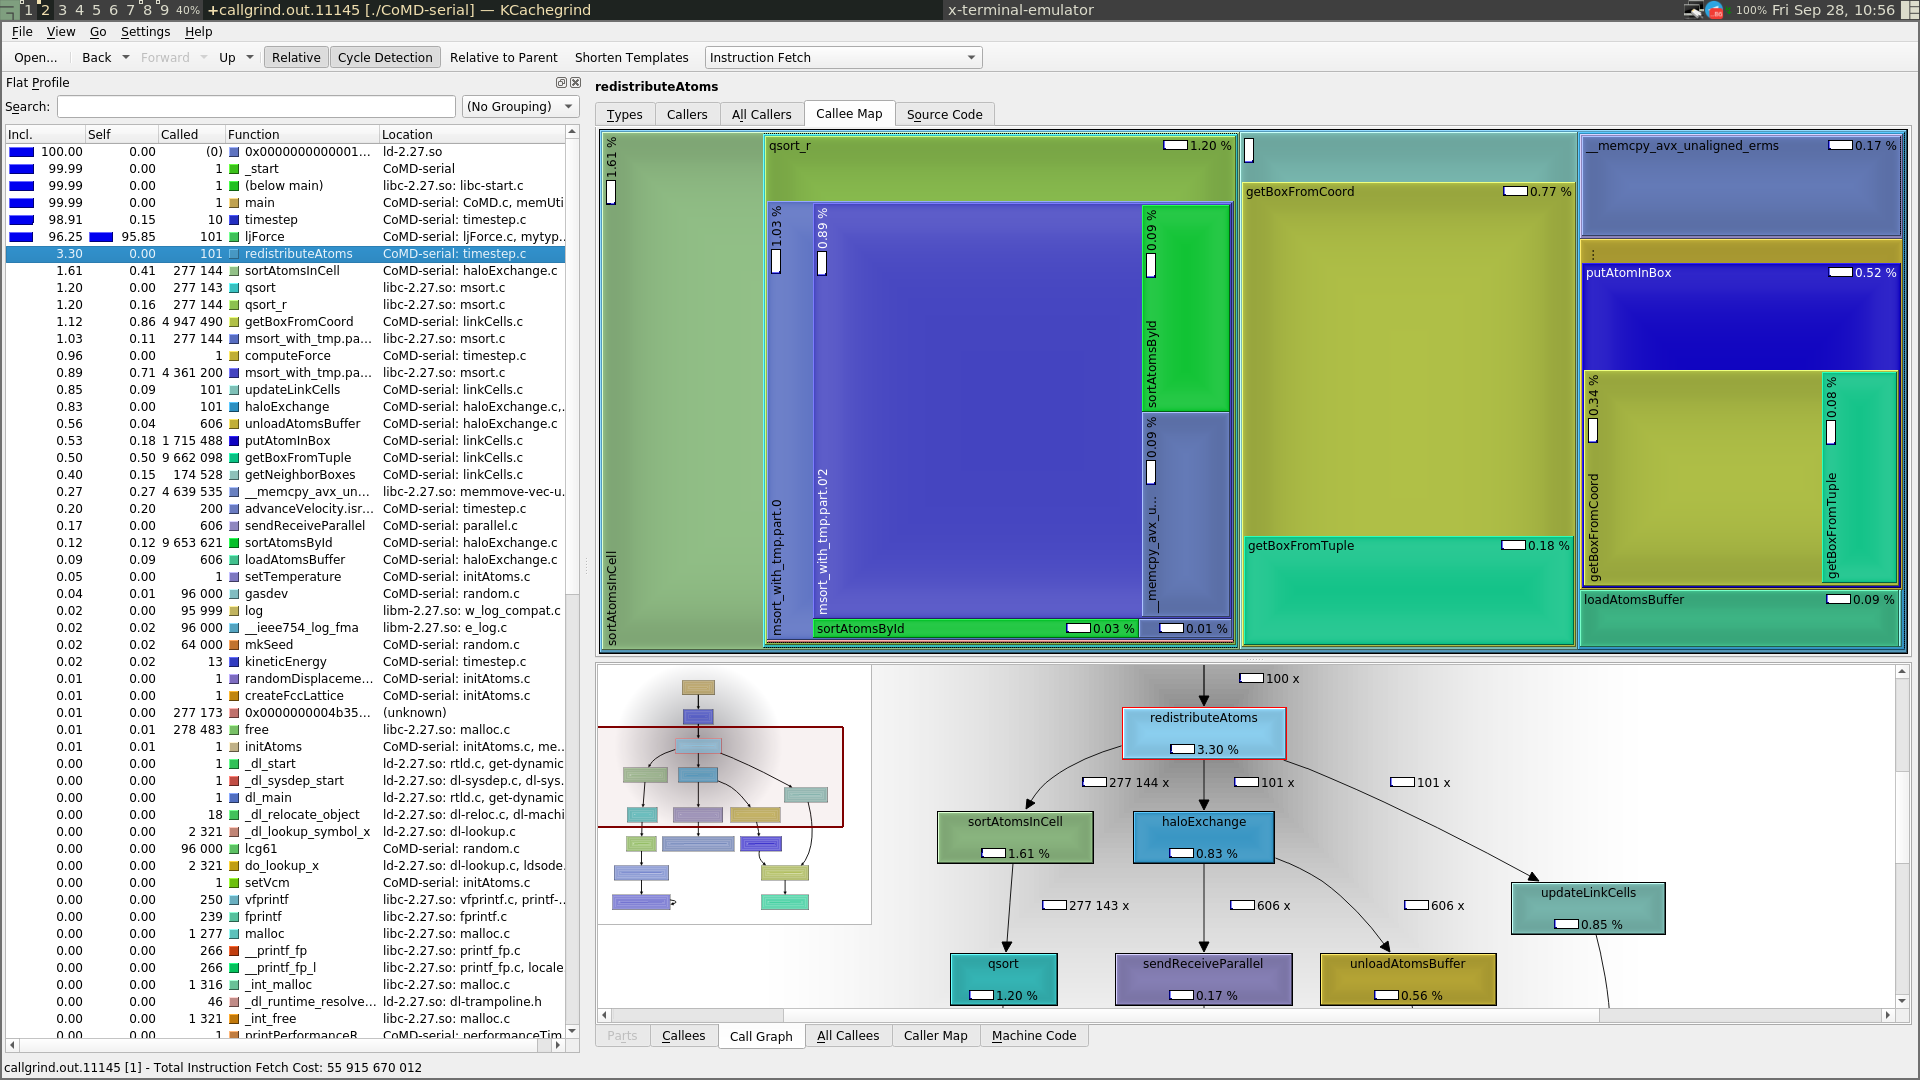
\includegraphics[height=.82\textheight]{kcachegrind}
    \caption{Flat profile, Call graph and Callee map in Kcachegrind}
  \end{figure}
}

\subsection{Cache profiling: analyzing locality and cache behavior}

\begin{frame}[fragile]{Valgrind: cache performance profiling with Cachegrind}

  \begin{description}
  \item[Cachegrind:] a cache and branch-prediction profiler
  \end{description}

  How to use it?
  \begin{itemize}
  \item Compile your code with {\tt -g} (debugging symbols
    $\Rightarrow$ line numbers)
  \item Launch cachegrind:
    \begin{lstlisting}
      valgrind --tool=cachegrind myprog <args>
    \end{lstlisting}
    \begin{itemize}
    \item[$\rightarrow$] a {\tt cachegrind.out.processid} file is
      generated
    \item<2>[$\rightarrow$] Optional parameter: {\tt
        --branch-sim=yes}\\
      Add info about branch (mis)prediction
    \end{itemize}
  \item Use {\tt cachegrind\_annotate} (CLI) or {\tt kcachegrind}
    (GUI) to analyze your profiling data:
    \begin{lstlisting}
      kcachegrind callgrind.out.processid
    \end{lstlisting}

    \begin{lstlisting}
      cg_annotate [--auto=yes] cachegrind.out.processid
    \end{lstlisting}
  \end{itemize}
\end{frame}

\begin{frame}[fragile]{Valgrind: cachegrind output}

  \begin{lstlisting}[style=valgrind,caption={Cachegrind
      output: recap}]

I   refs:   55,915,671,268
I1  misses:          5,140
LLi misses:          4,500
I1  miss rate:        0.00%
LLi miss rate:        0.00%

D   refs:   18,250,289,589  (14,026,926,013 rd + 4,223,363,576 wr)
D1  misses:     75,849,077  (    61,737,517 rd +    14,111,560 wr)
LLd misses:     24,401,720  (    12,382,283 rd +    12,019,437 wr)
D1  miss rate:         0.4% (           0.4%   +           0.3% )
LLd miss rate:         0.1% (           0.1%   +           0.3% )

LL refs:        75,854,217  (    61,742,657 rd +    14,111,560 wr)
LL misses:      24,406,220  (    12,386,783 rd +    12,019,437 wr)
LL miss rate:          0.0% (           0.0%   +           0.3% )
  \end{lstlisting}

\end{frame}

\begin{frame}[fragile]{Valgrind: cachegrind output}

  \begin{lstlisting}[style=valgrind,xleftmargin=-0.75cm,basicstyle=\tiny\ttfamily,caption={Cachegrind
      output: annotated output}]

% cg_annotate --auto=yes cachegrind.out.30363
--------------------------------------------------------------------------------
I1 cache:         32768 B, 64 B, 8-way associative
D1 cache:         32768 B, 64 B, 8-way associative
LL cache:         3145728 B, 64 B, 12-way associative

[...]

        Ir I1mr ILmr         Dr      D1mr    DLmr        Dw    D1mw   DLmw
[...]
11,770,984    0    0    554,288         0       0         0       0      0 for (int ii=begin, iTmp=0; ii<end; ++ii, ++iTmp)
         .    .    .          .         .       .         .       .      . {
24,854,584   11   11  5,192,632   560,752 512,730 4,915,488     302    201    tmp[iTmp].gid  = atoms->gid[ii];
15,023,608    0    0  5,192,632   560,752 518,652 4,915,488       0      0    tmp[iTmp].type = atoms->iSpecies[ii];
 9,830,976    0    0  4,915,488   892,840 779,741 4,915,488     101      1    tmp[iTmp].rx =   atoms->r[ii][0];
 9,830,976    0    0  4,915,488   514,662 217,133 4,915,488     101    101    tmp[iTmp].ry =   atoms->r[ii][1];
 9,830,976   11   11  4,915,488   615,696 473,665 4,915,488     101    100    tmp[iTmp].rz =   atoms->r[ii][2];
11,493,840    0    0  4,915,488   892,840 769,859 4,915,488     101    100    tmp[iTmp].px =   atoms->p[ii][0];
 9,830,976    0    0  4,915,488   514,662 229,502 4,915,488     101     99    tmp[iTmp].py =   atoms->p[ii][1];
 9,830,976    0    0  4,915,488   615,696 480,076 4,915,488     101      0    tmp[iTmp].pz =   atoms->p[ii][2];
         .    .    .          .         .       .         .       .      . }
   831,432    0    0          0         0       0   277,144       0      0 qsort(&tmp, nAtoms, sizeof(AtomMsg), sortAtomsById);
10,385,264    0    0    554,288         0       0         0       0      0 for (int ii=begin, iTmp=0; ii<end; ++ii, ++iTmp)
         .    .    .          .         .       .         .       .      . {
10,108,120   11   11  5,192,632         0       0 4,915,488       0      0    atoms->gid[ii]   = tmp[iTmp].gid;
10,939,552    0    0  5,192,632         0       0 4,915,488       0      0    atoms->iSpecies[ii] = tmp[iTmp].type;
29,492,928    0    0  4,915,488         0       0 4,915,488       0      0    atoms->r[ii][0]  = tmp[iTmp].rx;
 9,830,976    1    1  4,915,488         0       0 4,915,488       0      0    atoms->r[ii][1]  = tmp[iTmp].ry;

[...]
\end{lstlisting}

\end{frame}

\subsection{Memory profiling: Evaluating memory usage}

\begin{frame}[fragile]{Valgrind: detecting memory-related errors with
    Memcheck}

  \begin{description}
  \item[Memcheck:] The default tool, and the most popular
    \begin{itemize}
    \item[\checkmark] Easy way to detect and locate memory bugs
    \item[{\tt x}] Again: terribly slow!
    \item[{\tt x}] Second main drawback: some false positives!
    \end{itemize}
  \end{description}

  \pause

  How to use it?
  \begin{itemize}
  \item Compile your code with {\tt -g} (debugging symbols
    $\Rightarrow$ line numbers)
  \item Maybe a good idea to limit compiler opts: {\tt -O0 or -O1}
  \item Launch detailed memory leak detector ({\tt --leak-check=yes}):
    \begin{lstlisting}
      valgrind --leak-check=yes myprog <args>
    \end{lstlisting}
  \item Read the (verbose) output!
  \end{itemize}

  \pause

  \begin{exampleblock}{Objective}
    Try to make your program so clean that Memcheck reports no errors
  \end{exampleblock}
\end{frame}

\begin{frame}[fragile]{Valgrind: Memcheck example}

  \begin{lstlisting}[style=c,gobble=1]
    #include <stdlib.h>

    void f(void) {
      int *x = malloc(10 * sizeof(int));
      x[10] = 0;     // problem 1: heap block overrun
    }                // problem 2: memory leak -- x not freed

    int main(void) {
      f();
      return 0;
    }
  \end{lstlisting}

  \vspace*{-0.5cm}%
  \hspace{-0.6cm}%
  \begin{overprint}
    \onslide<1>
    \begin{lstlisting}[style=valgrind,gobble=6,caption={Valgrind output: Memcheck error}]
      ==19182== Invalid write of size 4
      ==19182==    at 0x804838F: f (example.c:6)
      ==19182==    by 0x80483AB: main (example.c:11)
      ==19182==  Address 0x1BA45050 is 0 bytes after a block of size 40 alloc'd
      ==19182==    at 0x1B8FF5CD: malloc (vg_replace_malloc.c:130)
      ==19182==    by 0x8048385: f (example.c:5)
      ==19182==    by 0x80483AB: main (example.c:11)
    \end{lstlisting}

    \onslide<2>
    \begin{lstlisting}[style=valgrind,gobble=6,
      caption={Valgrind output: Memory leaks messages}]
      ==19182== 40 bytes in 1 blocks are definitely lost in loss record 1 of 1
      ==19182==    at 0x1B8FF5CD: malloc (vg_replace_malloc.c:130)
      ==19182==    by 0x8048385: f (a.c:5)
      ==19182==    by 0x80483AB: main (a.c:11)
    \end{lstlisting}
  \end{overprint}

\end{frame}

\frame{
  \frametitle{Valgrind: Memcheck memory leaks report}

  Memcheck classifies memory leaks in 4 general types:
  \begin{description}
  \item[Still reachable] Not specially relevant
  \item[Definitely lost] Symptom of problems. This is a
    \underline{memory leak}
  \item[Indirectly lost] Problems usually caused by a previous
    definitely lost issue (that should be fixed earlier!)
  \item[Possibly lost] Inner pointers to allocated mem
    blocks. Investigate if not on purpose
  \end{description}

  \pause

  \begin{exampleblock}{Personally\ldots}
    I like achieving {\bf memcheck-clean} runs
  \end{exampleblock}
}

\frame{
  \frametitle{Valgrind: Memcheck can be used in parallel environments}

  \begin{itemize}
  \item {\bf Memcheck} can be used to debug and profile parallel
    programs: \emph{pthreads}, \emph{openmp}, even \emph{MPI}!
    \begin{itemize}
    \item usually increases the number of false positives!
    \end{itemize}
  \item Very good documentation: {\small \url{http://valgrind.org/docs/manual/mc-manual.html}}
  \end{itemize}
}

\frame{
  \frametitle{Valgrind + gdb}

  \begin{block}{GDB, the GNU Project debugger}
    allow us to see what is going on `inside' another program while
    it executes -- or what another program was doing at the moment it
    crashed.
  \end{block}

  \begin{itemize}
  \item To use {\tt valgrind} with {\tt gdb}:
    \begin{description}
    \item[{\tt --vgdb=<no|yes|full>} [default: yes]] ~\\
      Valgrind provides \emph{``gdbserver''} functionality, allowing
      an external GNU GDB debugger to control and debug your program
      when it runs on.
    \item[{\tt --vgdb-error=<number>} [default: 999999999]] ~\\
      Valgrind will wait for \emph{<number>} errors to be reported
      before freezing the program and waiting for a GDB connection.
    \end{description}
  \end{itemize}
}

\begin{frame}[fragile]{Valgrind: Massif, a heap profiler}

  \begin{quote}
    Heap profiling can help you reduce the amount of memory your
    program uses
  \end{quote}

  \pause

  How to use it?
  \begin{itemize}
  \item Again: compile your code with {\tt -g}
  \item Launch massif to gather heap profiling information:
    \begin{lstlisting}
      valgrind --tool=massif myprog <args>
    \end{lstlisting}
    \begin{itemize}
    \item[$\rightarrow$] a {\tt massif.out.processid} file is
      generated
    \item<3>[$\rightarrow$] key parameter: {\tt --time-unit=<i|ms|B>} [default: i]]\\
      The time unit used for the profiling:
      \begin{description}
      \item[i] instructions executed, good for most cases
      \item[ms] real (wallclock) time
      \item[B] bytes allocated/deallocated, useful for very short-run
        programs and testing purposes
      \end{description}
    \end{itemize}
  \item Use {\tt ms\_print} (CLI) to see the information gathered by
    Massif in an easy-to-read form (or {\tt massive\_visualizer} (GUI)
    \begin{lstlisting}
      ms_print massif.out.processid
    \end{lstlisting}
  \end{itemize}

\end{frame}

\begin{frame}[fragile]{Valgrind: massif output}

  \begin{lstlisting}[style=valgrind,xleftmargin=-0.75cm,basicstyle=\scriptsize\ttfamily,] 
   MB
3.952^                                                                    #
     |                                                                   @#:
     |                                                                 :@@#:
     |                                                            @@::::@@#:
     |                                                            @ :: :@@#::
     |                                                          @@@ :: :@@#::
     |                                                       @@:@@@ :: :@@#::
     |                                                    :::@ :@@@ :: :@@#::
     |                                                    : :@ :@@@ :: :@@#::
     |                                                  :@: :@ :@@@ :: :@@#::
     |                                                @@:@: :@ :@@@ :: :@@#:::
     |                           :       ::         ::@@:@: :@ :@@@ :: :@@#:::
     |                        :@@:    ::::: ::::@@@:::@@:@: :@ :@@@ :: :@@#:::
     |                     ::::@@:  ::: ::::::: @  :::@@:@: :@ :@@@ :: :@@#:::
     |                    @: ::@@:  ::: ::::::: @  :::@@:@: :@ :@@@ :: :@@#:::
     |                    @: ::@@:  ::: ::::::: @  :::@@:@: :@ :@@@ :: :@@#:::
     |                    @: ::@@:::::: ::::::: @  :::@@:@: :@ :@@@ :: :@@#:::
     |                ::@@@: ::@@:: ::: ::::::: @  :::@@:@: :@ :@@@ :: :@@#:::
     |             :::::@ @: ::@@:: ::: ::::::: @  :::@@:@: :@ :@@@ :: :@@#:::
     |           @@:::::@ @: ::@@:: ::: ::::::: @  :::@@:@: :@ :@@@ :: :@@#:::
   0 +----------------------------------------------------------------------->Mi
     0                                                                   626.4
 Number of snapshots: 63
 Detailed snapshots: [3, 4, 10, 11, 15, 16, 29, 33, 34, 36, 39, 41,
                      42, 43, 44, 49, 50, 51, 53, 55, 56, 57 (peak)]
  \end{lstlisting}
\end{frame}


\subsection{Profiling with {\tt perf}}

\frame{
  \frametitle{\insertsubsectionhead}

  \begin{block}{Perf}
    Linux profiling with performance counters

    \begin{itemize}
    \item Use of {\bf performance counters}~\footnote{CPU hardware
        registers that count hardware events such as instructions
        executed, cache-misses suffered, or branches mispredicted} to
      trace dynamic control flow and identify hotspots
    \item Use of {\bf tracepoints}~\footnote{Instrumentation points
        placed at logical locations in code, such as for system calls,
        TCP/IP events, file system operations, etc.} to collect useful
      information about the running processl, including timestamps and
      stack traces.
    \end{itemize}
  \end{block}
}

\frame{
  \frametitle{Perf interface}

  Simple to use CLI:
  \begin{description}[perf annotate:]
  \item[perf stat:] obtain event counts
  \item[perf record:] record events for later reporting
  \item[perf report:] break down events by process, function, etc.
  \item[perf annotate:] annotate assembly or source code with event
    counts
  \item[perf top:] see live event count
  \item[perf bench:] run different kernel microbenchmarks
  \end{description}

  $\Rightarrow$Good documentation: \url{https://perf.wiki.kernel.org}
}


\section{Optimization and Profiling of Parallel Code}

\subsection{Paraver et al: an overview}

\frame{
  \frametitle{Paraver et al: an overview of BSC Performance Tools}
  % \item ompP
  \begin{block}{Leveraging BSC's HPC Performance
      Tools~\footnote{Barcelona Supercomputing Center Performance
        Tools: \url{http://tools.bsc.es}\\~~~Repositories:
        \url{http://github.com/bsc-performance-tools}} to profile and
      optimize parallel applications}
    \begin{center}
      Basic toolchain:~~~~~~~~~~~~~~~~~~~~~~~~~~~~~~~~~~~~~~~~~~~~~~~~~~~~~~~~~~~~~~~~~
    \item Extrae $\Rightarrow$ Paraver $\Rightarrow$ Dimemás
    \end{center}
  \end{block}

  \begin{description}
  \item[Extrae:] package that generates Paraver-trace files for
    a post-morten analysis
  \item[Paraver:] trace visualization and analysis browser
  \item[Dimemás:] high-abstracted network simulator for message-passing programs
  \end{description}
}

\frame{
  \frametitle{BSC's performance analysis tools}

  Let's embrace again this \underline{core idea} (from a previous slide):

  \begin{block}{}
    \begin{quotation}
      Profile first, optimize later
    \end{quotation}
  \end{block}

  \begin{itemize}
  \item Analysis must be the first step towards the optimization of an
    application
  \item Performance analysis tools allow us to identify and
    characterize the inefficiencies that cause a poor performance
  \end{itemize}

  \pause

  \begin{block}{BSC's toolchain main objectives:}
    \begin{itemize}
    \item flexibility and versatility: platforms, environments,
      programming models\ldots
    \item simplify and facilitate the process of extracting information from the performance data
    \end{itemize}
  \end{block}
}


\subsection{Dynamic instrumentation to trace programs with {\tt
    extrae}}

\frame{
  \frametitle{Extrae}

  {\bf Extrae}: dynamic instrumentation package to trace programs
  \begin{itemize}
  \item Generates trace files that can be later visualized with {\bf
      Paraver}
  \item Works with different programming models:
    \begin{itemize}
    \item shared memory model (such as OpenMP and pthreads)
    \item the message passing (MPI)
    \item hybrid
    \end{itemize}
  \end{itemize}
}

\frame{
  \frametitle{Extrae: main features}

  \begin{itemize}
  \item Parallel programming models \tikzmark{start}
    \begin{itemize}
    \item MPI, OpenMP, pthreads, OmpSs, CUDA, OpenCL,\\ Java, Python\ldots
    \end{itemize}
  \item Platforms
    \begin{itemize}
    \item Intel, Cray, BlueGene, MIC, ARM, Android,\\ Fujitsu Spark\ldots
    \end{itemize}
  \item Hardware Performance Counters
    \begin{itemize}
    \item Using PAPI interface
    \end{itemize}
  \item Link to source code
    \begin{itemize}
    \item Callstack at MPI routines
    \item OpenMP outlined routines
    \item Selected user functions (Dyninst)
    \end{itemize}
  \item Periodic sampling \tikzmark{end}
  \item User events (Extrae API)
  \end{itemize}

  \begin{tikzpicture}[remember picture,overlay]
    \draw[decorate,decoration={calligraphic brace}]
    ([yshift=10pt,xshift=150pt]{{pic cs:end}|-{pic cs:start}}) --
    node[xshift=5pt,anchor=west] {\parbox{5cm}{No need to\\ recompile/link!}}
    ([xshift=150pt]{pic cs:end})
    ;
  \end{tikzpicture}
}

\frame{
  \frametitle{Extrae: how it works}

  \begin{itemize}
  \item Symbol substitution through LD\_PRELOAD \hfill \alert{\bf $\leftarrow$ Recommended!}
    \begin{itemize}
    \item Specific \underline{tracing libraries} for each combination of runtimes
      \begin{itemize}
      \item MPI
      \item OpenMP
      \item OpenMP+MPI
      \item \ldots
      \end{itemize}
    \end{itemize}
  \item Dynamic instrumentation
    \begin{itemize}
    \item Based on DynInst (developed by U.Wisconsin/U.Maryland)
      \begin{itemize}
      \item Instrumentation in memory
      \item Binary rewriting
      \end{itemize}
    \end{itemize}
  \item Alternatives
    \begin{itemize}
    \item Static link (i.e., PMPI, Extrae API)
    \end{itemize}
  \end{itemize}
}

\frame{
  \frametitle{Extrae: typical scenario}

  \begin{itemize}
  \item Traces are obtained with {\bf Extrae} in a Supercomputer
    running the code to optimize:
    \begin{itemize}
    \item using the {\tt LD\_PRELOAD} mechanism to intercept entries and
      exits to MPI
    \item data from hardware counters (cache misses, instructions and
      cycles) at those points
    \end{itemize}
  \item Traces are analysed post-mortem in a PC with {\bf Paraver},
    and maybe also with {\bf Dimemas}
  \item Batch analysis possibility: {\bf Paramedir}
  \end{itemize}
}

\frame{
  \frametitle{Extrae: how to use it}

  In a nutshell:
  \begin{enumerate}
  \item Adapt the job submission script
  \item \structure{[optional]} Tune the Extrae XML configuration file
    \begin{itemize}
    \item Examples distributed with Extrae:\\
      \hfill {\footnotesize \tt \$\{EXTRAE\_HOME\}/share/example}~\footnote{In
        Finisterrae II:\\~~~{\scriptsize
          EXTRAE\_HOME=/opt/cesga/easybuild-cesga/software/MPI/gcc/6.4.0/openmpi/2.1.1/extrae/3.5.2}}
    \end{itemize}
  \item Submit/Run the job to generate the trace
  \end{enumerate}

  \pause

  All details in Extrae official documentation:
  {\small \url{https://tools.bsc.es/sites/default/files/documentation/pdf/extrae-3.5.2-user-guide.pdf}}
}

\begin{frame}[fragile]{Extrae: submission script}

  \vspace*{-0.2cm}
  \begin{lstlisting}[style=shell,gobble=3,caption={submit\_trace.sh}]
    #!/bin/sh
    #SBATCH -t 00:20:00 # execution time hh:mm:ss *OB*
    #SBATCH -n 16 #tasks (MPI processes)
    #SBATCH -c 24 #cores/task (shared-mem threads/process)
    ##SBATCH -N 16  #nodes
    #SBATCH -p cola-corta

    @module load gcc/6.4.0 openmpi/2.1.1 extrae/3.5.2
    # export TRACE_NAME=trace_filename.prv # *OP*
    @
    srun -n 16 @${HOME}/trace.sh@ parallel_binary [params]
  \end{lstlisting}

  \pause

  \vspace*{-0.2cm}
  \begin{lstlisting}[style=shell,gobble=3,caption={trace.sh}]
    #!/bin/sh
    source /opt/cesga/easybuild-cesga/software/MPI/gcc/6.4.0\
                    /openmpi/2.1.1/extrae/3.5.2/etc/extrae.sh
    ¿export EXTRAE_CONFIG_FILE=${HOME}/extrae.xml¿
    ¿export LD_PRELOAD=${EXTRAE_HOME}/lib/libmpitrace.so¿ # C code

    $*     # Run the program
  \end{lstlisting}
\end{frame}

\frame{
  \frametitle{Extrae: tracing library to use}

  \begin{table}
    \caption{Tracing libraries~\footnote{Include suffix `f' for Fortran
        codes} to use with {\tt LD\_PRELOAD}}
    \rowcolors{2}{}{gray!20}
    \begin{tabular}{lccccc}
      {\bf Library} & {\bf Serial} & {\bf MPI} & {\bf OpenMP} & {\bf pthreads} & {\bf CUDA}\\
      libseqtrace & \structure{\checkmark} & & & & \\
      libmpitrace[f] & & \structure{\checkmark} & & & \\
      libomptrace & & & \structure{\checkmark} & & \\
      libpttrace & & & & \structure{\checkmark} & \\
      libcudatrace & & & & & \structure{\checkmark}\\
      libompitrace[f] & & \structure{\checkmark} & \structure{\checkmark} & & \\
      libptmpitrace[f] & & \structure{\checkmark} & & \structure{\checkmark} & \\
      libcudampitrace[f] & & \structure{\checkmark} & & & \structure{\checkmark}\\
    \end{tabular}
  \end{table}
}

\frame{
  \frametitle{Extrae: XML configuration}

  See examples in {\tt \$\{EXTRAE\_HOME\}/share/example}

  For example:
  \begin{itemize}
  \item for MPI + OpenMP:\\
    {\tt \$\{EXTRAE\_HOME\}/share/example/MPI+OMP/extrae.xml}
  \item only MPI:\\
    {\tt \$\{EXTRAE\_HOME\}/share/example/MPI/extrae.xml}
  \item only OpenMP:\\
    {\tt \$\{EXTRAE\_HOME\}/share/example/OMP/extrae.xml}
  \end{itemize}
}

\frame{
  \frametitle{Extrae: XML configuration, easy to customize (i)}

  \begin{figure}
    \hspace*{-0.5cm}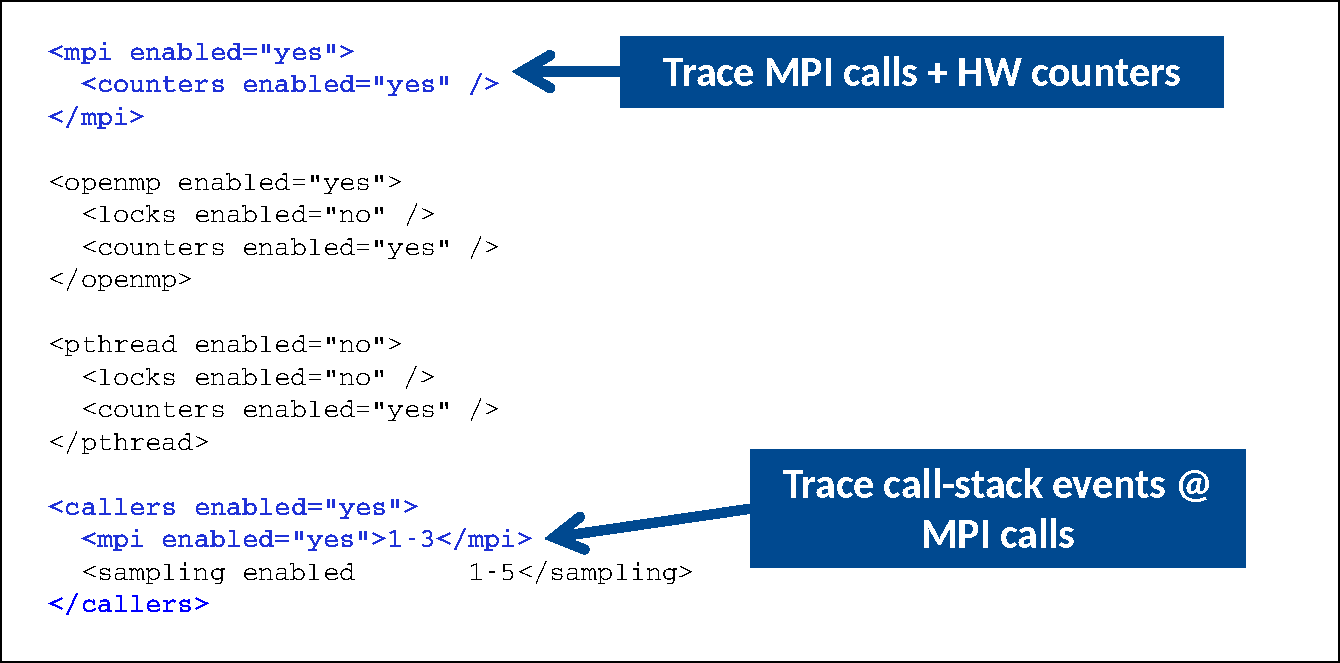
\includegraphics[width=1.1\textwidth]{extraexml1}
  \end{figure}
}

\frame{
  \frametitle{Extrae: XML configuration, easy to customize (ii)}

  \begin{figure}
    \hspace*{-.8cm}\includegraphics[width=1.15\textwidth]{extraexml2}
  \end{figure}
}

\frame{
  \frametitle{Extrae: XML configuration, easy to customize (iii)}

  \begin{figure}
    \hspace*{-0.5cm}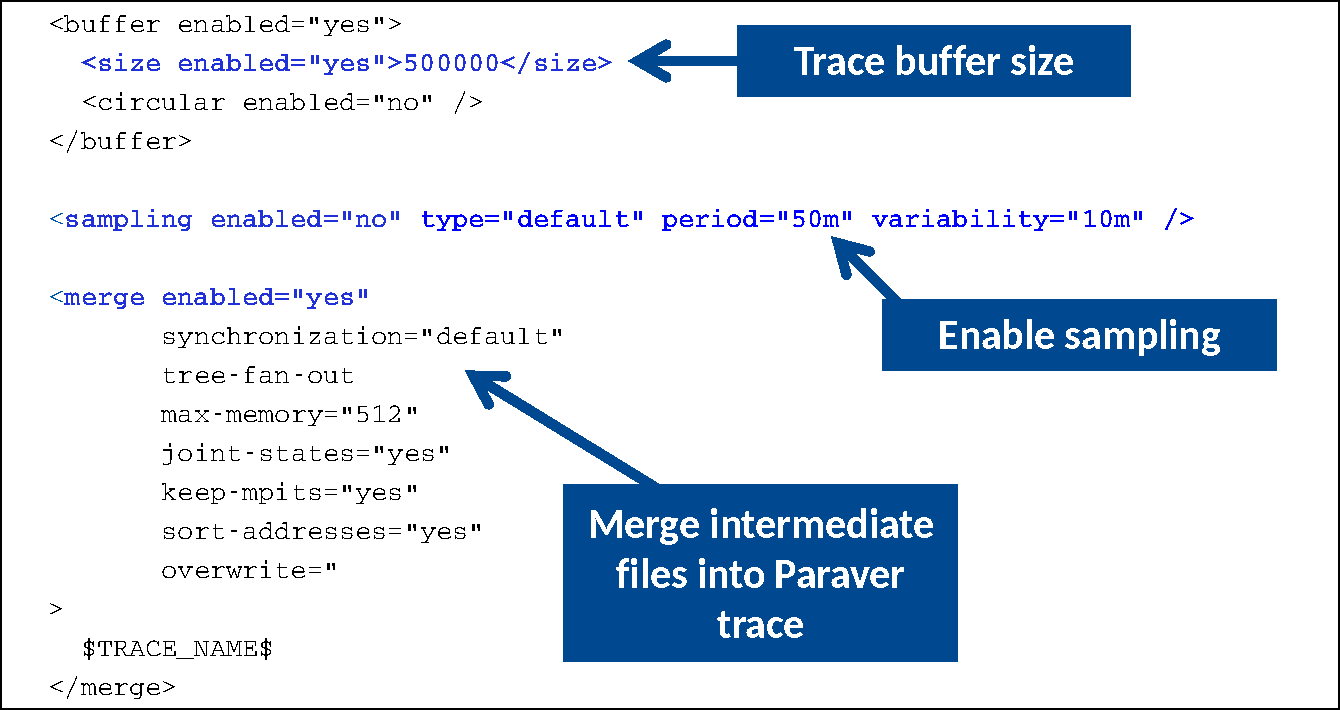
\includegraphics[width=1.1\textwidth]{extraexml3}
  \end{figure}
}

\begin{frame}[fragile]{Extrae: job sumission and trace files}
  \begin{enumerate}
  \item Submit your job!
    \begin{lstlisting}[style=shell,gobble=5]
      sbatch submit_trace.sh   # FT2 submission using SLURM
    \end{lstlisting}
  \item Once finished, the trace is provided in 3 files
    \begin{lstlisting}[style=shell,gobble=5]
      trace_filename.pcv
      trace_filename.prv         # <- the one used by Paraver
      trace_filename.row
    \end{lstlisting}
  \end{enumerate}
\end{frame}

\subsection{Performance analysis with {\tt paraver}}

\frame{
  \frametitle{Paraver}

  {\bf Paraver}: a flexible performance analysis tool
  \begin{itemize}
  \item Core component in BSC's toolchain
  \item Key design concept:
    \begin{itemize}
    \item provide a qualitative global perception of the application
      behavior by visual inspection
    \item then, focus on the detailed quantitative analysis of the problems
    \end{itemize}

    \pause

  \item Main features: flexible and versatile.\\
    Two main pillars:
    \begin{itemize}
    \item agnostic trace format (no semantics on it)
    \item metrics are not hardwired on the tool but programmed
    \end{itemize}

    \pause

  \item Other features:
    \begin{itemize}
    \item detailed quantitative analysis of program performance
    \item concurrent comparative analysis of several traces
    \item customizable semantics of the visualized information
    \item cooperative work, sharing views of the tracefile
    \item building of derived metrics
    \end{itemize}
  \end{itemize}
}

\frame{
  \frametitle{Paraver: views}

  Two main displays to provide performance information:
  \begin{description}
  \item[Timeline:]
    Behavior of application along time and processes
    \begin{figure}
      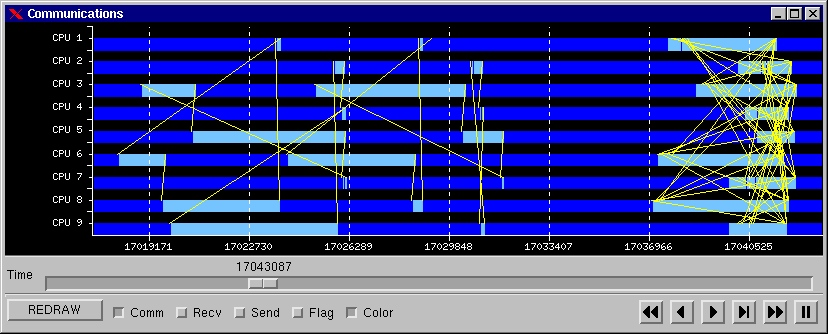
\includegraphics[width=0.7\textwidth]{paravertimeline}
    \end{figure}

    \pause

  \item[Tables:] Numerical analysis of the data
    \begin{itemize}
    \item Profiles, histograms, correlations
    \end{itemize}
    \begin{figure}
      \hspace*{-0.5cm}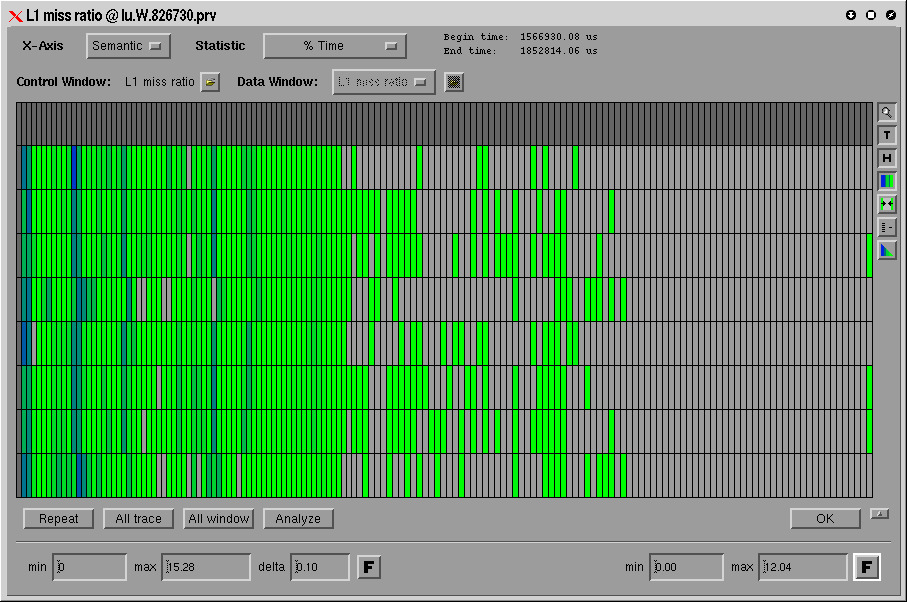
\includegraphics[width=0.4\textwidth]{paraverhistogram}
      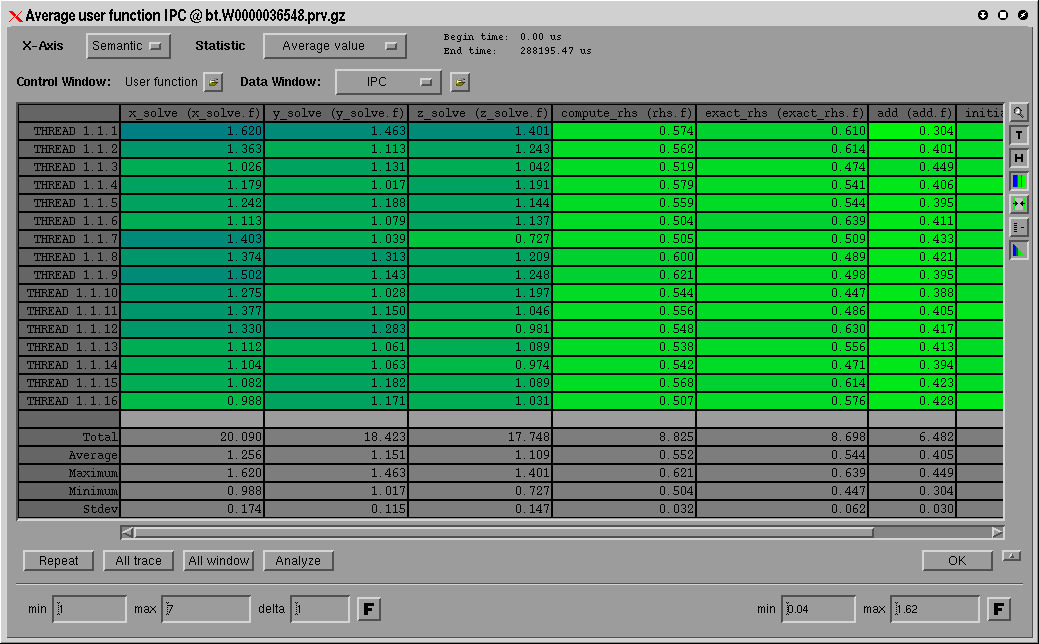
\includegraphics[width=0.43\textwidth]{paraverdata}
    \end{figure}
  \end{description}
}

\frame{
  \frametitle{Paraver, a performance data browser}

  \begin{figure}
    \includegraphics[width=\textwidth]{paraverworkflow}
  \end{figure}
}

\frame{
  \frametitle{Paraver: Profiles, histograms, correlations}

  \begin{figure}
    \hspace*{-0.5cm}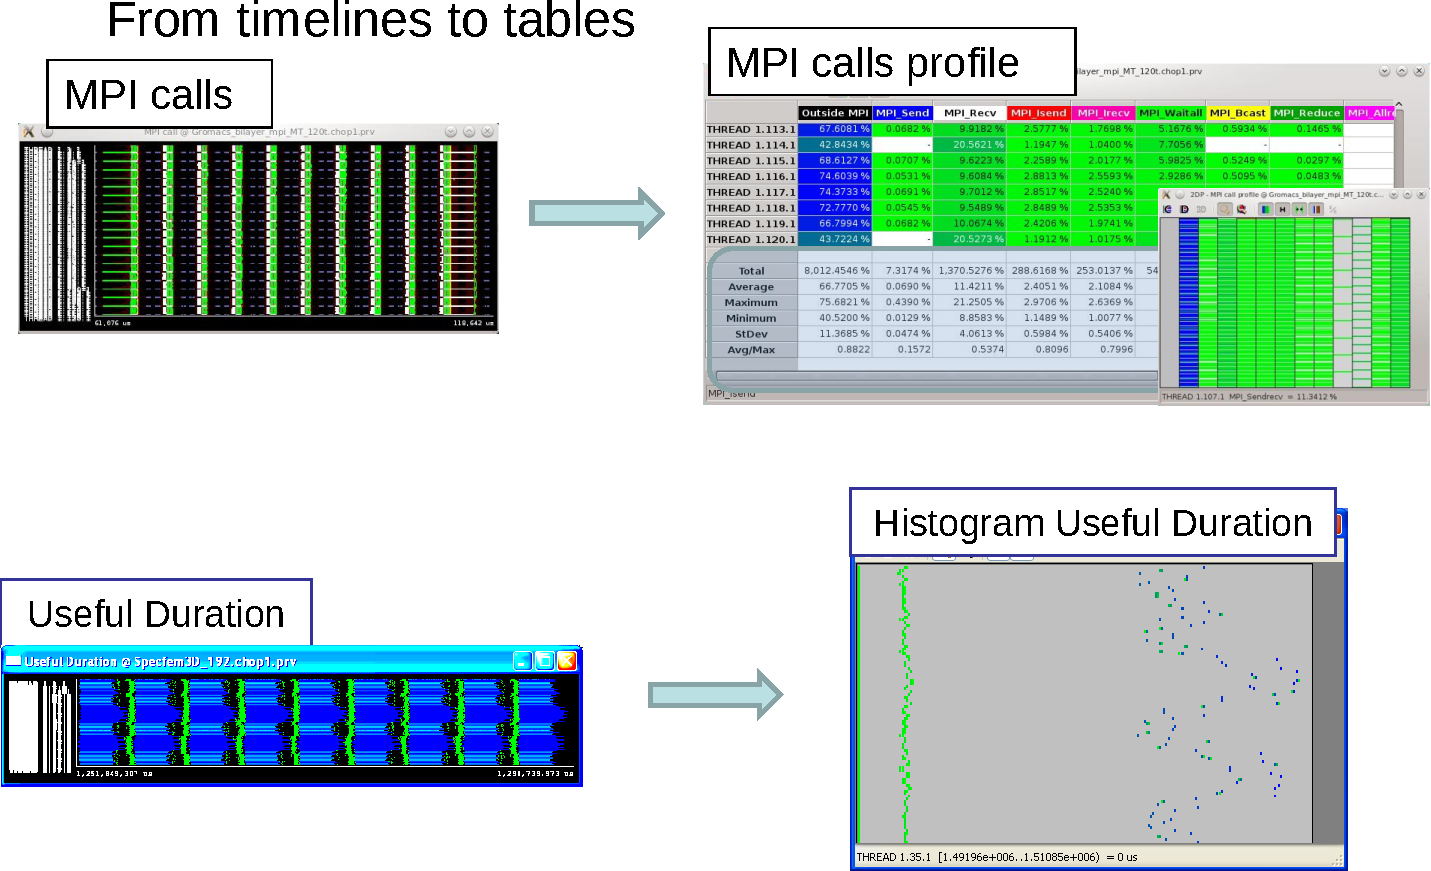
\includegraphics[width=1.1\textwidth]{paravercor}
  \end{figure}
}

\frame{
  \frametitle{Paraver: Analyzing variability through histograms and timelines}

  Key idea in {\tt paraver}: {\bf Gradient}

  \vspace*{-0.3cm}
  \begin{figure}
    \hspace*{-0.5cm}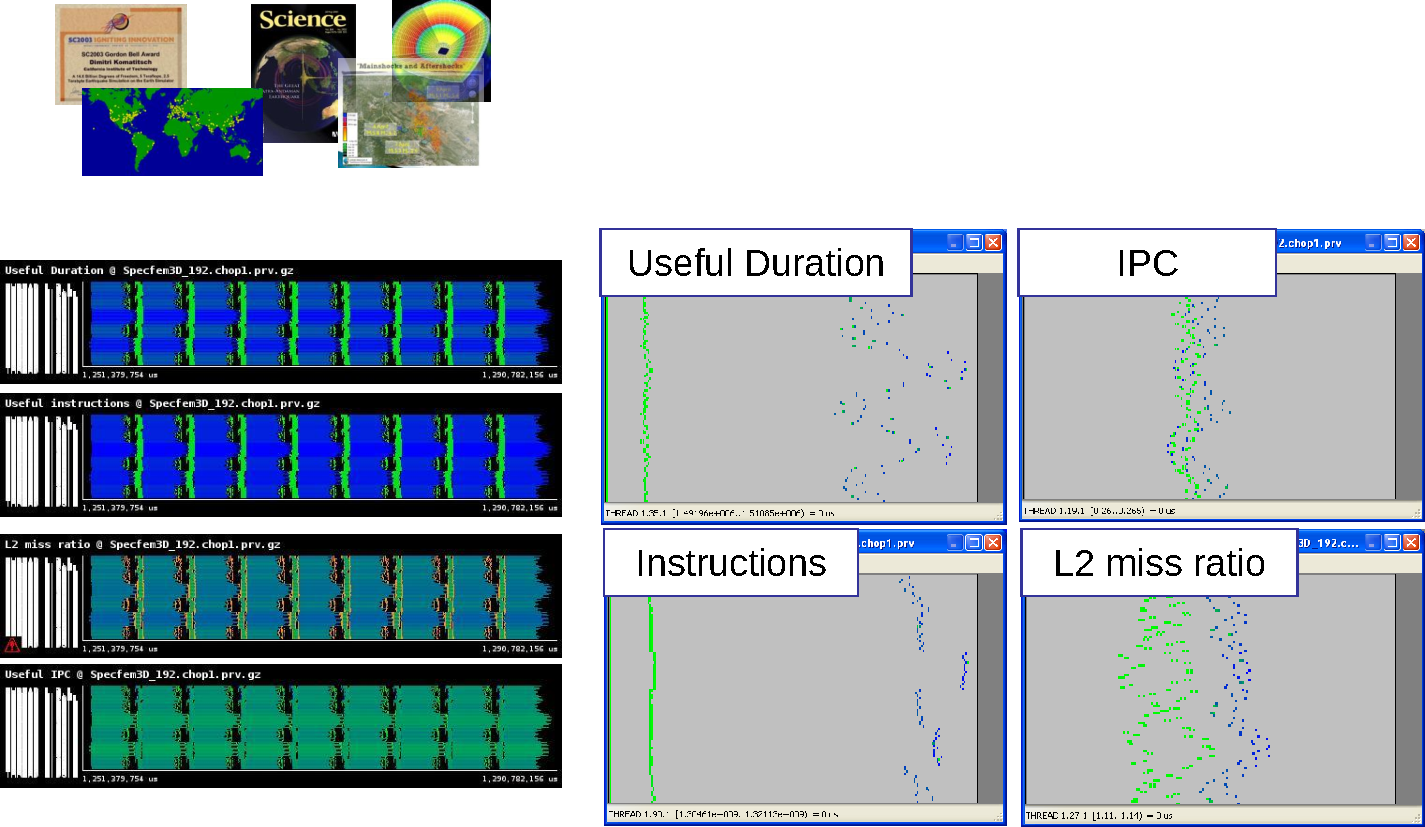
\includegraphics[width=1.1\textwidth]{paraveranal}
  \end{figure}
}

\frame{
  \frametitle{Paraver: Improvement after detecting imbalances}

  After some months of hard work\ldots\footnote{Real experience from a
    BSC experiment}

  \begin{figure}
    \hspace*{-0.8cm}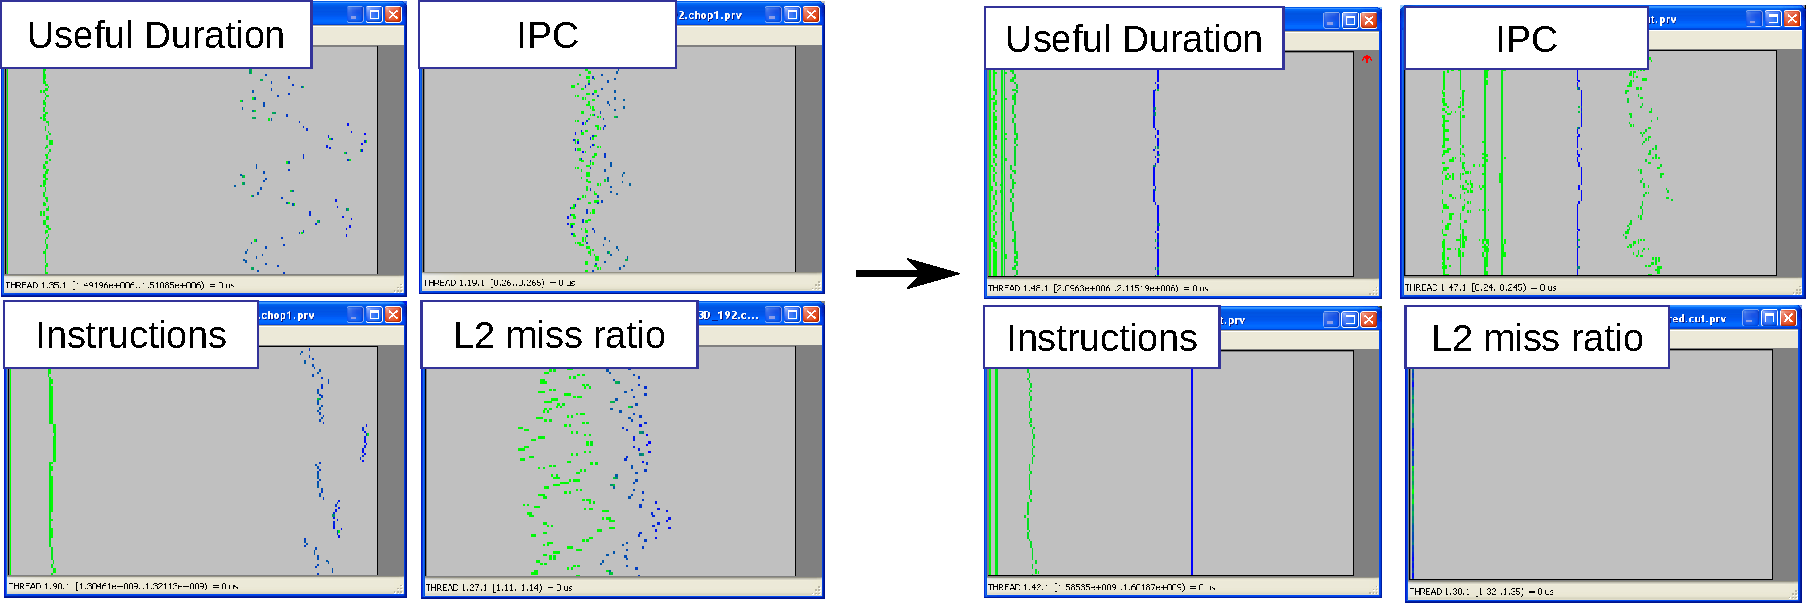
\includegraphics[width=1.15\textwidth]{paraverimprove}
  \end{figure}
}

\frame{
  \frametitle{Paraver: From tables to timelines}

  Where in the timeline do the values in certain table columns appear?
  \vspace*{-0.5cm}
  \begin{itemize}
  \item for example, I want to see the time distribution of a given routine
  \end{itemize}
  \vspace*{-0.2cm}
  \begin{figure}
    \hspace*{-0.8cm}\includegraphics[width=1.15\textwidth]{paravertables}
  \end{figure}
}

\begin{frame}[fragile]{Install {\tt paraver} in your computer}
  \begin{itemize}
  \item Download {\tt paraver} from the official site:\\
    \hfil \url{https://tools.bsc.es/downloads}
  \item Download the tutorials and uncompress them into the {\tt
      paraver} directory:\\
    \hfil \url{https://tools.bsc.es/paraver-tutorials}
  \item Launch paraver. For example: (use your installation path)
    \begin{lstlisting}[style=shell,gobble=3]
      /opt/wxparaver-4.7.2-Linux_x86_64/bin/wxparaver
    \end{lstlisting}
  \item Check the tutorials: {\small (also available in pdf and html)}\\
    \hfil Help$\rightarrow$Tutorials
  \end{itemize}
\end{frame}

%\section{Parametric analysis of behaviour with {\tt dimemas}}

%\begin{frame}
%\end{frame}

\appendix

\begin{frame}[allowframebreaks]{References}

  \nocite{*}
  \bibliography{slides}
  \bibliographystyle{abbrv}

\end{frame}

\end{document}